%% Version 4.3.2, 25 August 2014
%DIF LATEXDIFF DIFFERENCE FILE
%DIF DEL short18_seabreeze_verification_submitted.tex   Fri Feb 14 13:28:57 2020
%DIF ADD short18_seabreeze_verification.tex             Fri Feb 14 14:52:37 2020
%
%%%%%%%%%%%%%%%%%%%%%%%%%%%%%%%%%%%%%%%%%%%%%%%%%%%%%%%%%%%%%%%%%%%%%%
% Template.tex --  LaTeX-based template for submissions to the 
% American Meteorological Society
%
% Template developed by Amy Hendrickson, 2013, TeXnology Inc., 
% amyh@texnology.com, http://www.texnology.com
% following earlier work by Brian Papa, American Meteorological Society
%
% Email questions to latex@ametsoc.org.
%
%%%%%%%%%%%%%%%%%%%%%%%%%%%%%%%%%%%%%%%%%%%%%%%%%%%%%%%%%%%%%%%%%%%%%
% PREAMBLE
%%%%%%%%%%%%%%%%%%%%%%%%%%%%%%%%%%%%%%%%%%%%%%%%%%%%%%%%%%%%%%%%%%%%%

%% Start with one of the following:
% DOUBLE-SPACED VERSION FOR SUBMISSION TO THE AMS
\documentclass{ametsoc}

% TWO-COLUMN JOURNAL PAGE LAYOUT---FOR AUTHOR USE ONLY
% \documentclass[twocol]{ametsoc}

%%%%%%%%%%%%%%%%%%%%%%%%%%%%%%%%
%%% To be entered only if twocol option is used

\journal{waf}

%  Please choose a journal abbreviation to use above from the following list:
% 
%   jamc     (Journal of Applied Meteorology and Climatology)
%   jtech     (Journal of Atmospheric and Oceanic Technology)
%   jhm      (Journal of Hydrometeorology)
%   jpo     (Journal of Physical Oceanography)
%   jas      (Journal of Atmospheric Sciences)	
%   jcli      (Journal of Climate)
%   mwr      (Monthly Weather Review)
%   wcas      (Weather, Climate, and Society)
%   waf       (Weather and Forecasting)
%   bams (Bulletin of the American Meteorological Society)
%   ei    (Earth Interactions)

%%%%%%%%%%%%%%%%%%%%%%%%%%%%%%%%
%Citations should be of the form ``author year''  not ``author, year''
\bibpunct{(}{)}{;}{a}{}{,}

%%%%%%%%%%%%%%%%%%%%%%%%%%%%%%%%

%%% To be entered by author:

%% May use \\ to break lines in title:

\title{Verifying Operational Forecasts of Land-Sea Breeze and Boundary Layer Mixing Processes}

%%% Enter authors' names, as you see in this example:
%%% Use \correspondingauthor{} and \thanks{Current Affiliation:...}
%%% immediately following the appropriate author.
%%%
%%% Note that the \correspondingauthor{} command is NECESSARY.
%%% The \thanks{} commands are OPTIONAL.

    %\authors{Author One\correspondingauthor{Author One, 
    % American Meteorological Society, 
    % 45 Beacon St., Boston, MA 02108.}
% and Author Two\thanks{Current affiliation: American Meteorological Society, 
    % 45 Beacon St., Boston, MA 02108.}}

\authors{Ewan Short\correspondingauthor{School of Earth Sciences, The University of Melbourne, Melbourne, Victoria, Australia.}} 

\email{shorte1@student.unimelb.edu.au}

%% Follow this form:
    % \affiliation{American Meteorological Society, 
    % Boston, Massachusetts.}

\affiliation{School of Earth Sciences, and ARC Centre of Excellence for Climate Extremes, The University of Melbourne, Melbourne, Victoria, Australia.}

%% Follow this form:
    %\email{latex@ametsoc.org}

%\email{}

%% If appropriate, add additional authors, different affiliations:
    %\extraauthor{Extra Author}
    %\extraaffil{Affiliation, City, State/Province, Country}

\DeclareMathOperator{\mse}{mse} 
\DeclareMathOperator{\cov}{cov} 
\DeclareMathOperator{\var}{var} 
\DeclareMathOperator{\pr}{Pr} 

%\extraauthor{}
%\extraaffil{}

%% May repeat for a additional authors/affiliations:

%\extraauthor{}
%\extraaffil{}

%%%%%%%%%%%%%%%%%%%%%%%%%%%%%%%%%%%%%%%%%%%%%%%%%%%%%%%%%%%%%%%%%%%%%
% ABSTRACT
%
% Enter your abstract here
% Abstracts should not exceed 250 words in length!
%
% For BAMS authors only: If your article requires a Capsule Summary, please place the capsule text at the end of your abstract
% and identify it as the capsule. Example: This is the end of the abstract. (Capsule Summary) This is the capsule summary.

% Run "latexdiff --append-context2cmd="abstract" short18_diurnal_cycles_winds.tex short18_diurnal_cycles_winds_revised.tex > short18_diurnal_cycles_winds_tracked_changes.tex" to track changes

%DIF 111c111
%DIF < \abstract{Forecasts issued by the Australian Bureau of Meteorology (BoM) are based on automated post-processed model data that is edited by human forecasters. Two types of edits are commonly made to the wind fields. These edits aim to improve how the influences of boundary layer mixing and land-sea breeze processes are represented in the forecast. In this study we compare the diurnally varying component of the BoM's official edited wind forecast, with that of station observations and unedited model datasets, to assess changes to error and bias resulting from these edits. We consider coastal locations across Australia over June, July and August 2018, aggregating data over three spatial scales. The edited forecast generally only produces a lower mean absolute error than model guidance at the coarsest spatial scale (over fifty thousand square kilometres), but can achieve lower seasonal biases over all spatial scales. However, the edited forecast only reduces errors or biases at particular times and locations, and rarely produces lower errors or biases than all model guidance products simultaneously. To better understand the biases in the diurnal wind cycles, we fit modified ellipses to the temporal hodographs of seasonally averaged diurnal wind cycles. Biases in the official forecast diurnal cycle vary with location for multiple reasons, including biases in the directions sea-breezes approach coastlines, amplitude and shape biases in the hodographs, and disagreement as to whether sea-breeze or boundary layer mixing processes contribute most to the diurnal cycle.}
%DIF -------
\abstract{Forecasters working for Australia's Bureau of Meteorology (BoM) produce a seven day forecast in two key steps: first they choose a model guidance dataset to base the forecast on, then they use graphical software to manually edit this data. Two types of edits are commonly made to the wind fields that aim to improve how the influences of boundary layer mixing and land-sea breeze processes are represented in the forecast. In this study I compare the diurnally varying component of the BoM's official wind forecast, with that of station observations and unedited model guidance datasets. I consider coastal locations across Australia over June, July and August 2018, aggregating data over three spatial scales. The edited forecast generally only produces a lower mean absolute error than model guidance at the coarsest spatial scale (over fifty thousand square kilometres), but can achieve lower seasonal biases over all spatial scales. However, the edited forecast only reduces errors or biases at particular times and locations, and rarely produces lower errors or biases than all model guidance products simultaneously. To better understand physical reasons for biases in the mean diurnal wind cycles, I fit modified ellipses to the seasonally averaged diurnal wind temporal hodographs. Biases in the official forecast diurnal cycle vary with location for multiple reasons, including biases in the directions sea-breezes approach coastlines, amplitude  biases, and disagreement in the relative contribution of sea-breeze and boundary layer mixing processes to the mean diurnal cycle.} %DIF > 
%DIF -------

\usepackage{comment}
%DIF PREAMBLE EXTENSION ADDED BY LATEXDIFF
%DIF UNDERLINE PREAMBLE %DIF PREAMBLE
\RequirePackage[normalem]{ulem} %DIF PREAMBLE
\RequirePackage{color}\definecolor{RED}{rgb}{1,0,0}\definecolor{BLUE}{rgb}{0,0,1} %DIF PREAMBLE
\providecommand{\DIFadd}[1]{{\protect\color{blue}\uwave{#1}}} %DIF PREAMBLE
\providecommand{\DIFdel}[1]{{\protect\color{red}\sout{#1}}}                      %DIF PREAMBLE
%DIF SAFE PREAMBLE %DIF PREAMBLE
\providecommand{\DIFaddbegin}{} %DIF PREAMBLE
\providecommand{\DIFaddend}{} %DIF PREAMBLE
\providecommand{\DIFdelbegin}{} %DIF PREAMBLE
\providecommand{\DIFdelend}{} %DIF PREAMBLE
%DIF FLOATSAFE PREAMBLE %DIF PREAMBLE
\providecommand{\DIFaddFL}[1]{\DIFadd{#1}} %DIF PREAMBLE
\providecommand{\DIFdelFL}[1]{\DIFdel{#1}} %DIF PREAMBLE
\providecommand{\DIFaddbeginFL}{} %DIF PREAMBLE
\providecommand{\DIFaddendFL}{} %DIF PREAMBLE
\providecommand{\DIFdelbeginFL}{} %DIF PREAMBLE
\providecommand{\DIFdelendFL}{} %DIF PREAMBLE
%DIF END PREAMBLE EXTENSION ADDED BY LATEXDIFF

\begin{document}

\maketitle

\section{Introduction}
\label{Sec:Introduction}
Modern weather forecasts are typically produced by models in conjunction with human forecasters. \DIFdelbegin \DIFdel{Forecasters }\DIFdelend \DIFaddbegin \DIFadd{Operational forecasters }\DIFaddend working for the Australian Bureau of Meteorology (BoM) \DIFaddbegin \DIFadd{undertake two key steps to }\DIFaddend construct a seven day forecast\DIFdelbegin \DIFdel{by loading model data into a software package called }\DIFdelend \DIFaddbegin \DIFadd{.
}

\DIFadd{First, they choose a }\textit{\DIFadd{model guidance}} \DIFadd{dataset on which to base the official forecast. Datasets from both the BoM and international modelling centres are available to Australia forecasters, with the BoM's Operational Consensus Forecast (OCF) an increasingly common choice. Australian forecasters themselves are rarely directly involved in model setup or post-processing, modelling is instead performed by other teams either within the BoM or internationally. Once the forecaster makes a choice of model guidance, the data is loaded into }\DIFaddend the Graphical Forecast Editor (GFE) \DIFdelbegin \DIFdel{, then editing this model data using tools within the GFE. Forecasters working for the United States National Weather Service also use GFE and utilise a similar approach. Forecasters can choose which model to base their forecast on, and refer to this as a choice of }\textit{\DIFdel{model guidance}}%DIFAUXCMD
\DIFdel{. Edits are typically made to account for }\DIFdelend \DIFaddbegin \DIFadd{software package. 
}

\DIFadd{In the second step, the forecaster uses GFE to }\textit{\DIFadd{manually edit}} \DIFadd{the model guidance data. Such edits aim to incorporate }\DIFaddend processes that are under-resolved at the resolutions of the model guidance products, or to correct for perceived biases of the model guidance being used. \DIFdelbegin \DIFdel{In Australia, the resulting gridded forecast datasets are provided to the public through the BoM's online MetEye data browser \mbox{%DIFAUXCMD
\citep{bomMetEye19}}\hspace{0pt}%DIFAUXCMD
, and are also translated into text and icon forecasts algorithmically. 
}%DIFDELCMD < 

%DIFDELCMD < %%%
\DIFdel{Forecasters , and the weather services that employ them, have good reasons for ensuring the diurnally varying component of their wind forecasts are as accurate as possible. In addition to the significant contribution diurnal wind cycles make to overall wind fields \mbox{%DIFAUXCMD
\citep[e.g.][]{dai99}}\hspace{0pt}%DIFAUXCMD
, diurnal wind cycles are important for the ventilation of pollution, with sea-breezes transporting clean maritime air inland, where it helps flush polluted air out of the boundary layer \mbox{%DIFAUXCMD
\citep{miller03, physick92}}\hspace{0pt}%DIFAUXCMD
. Furthermore, diurnal wind cycles affect the function of wind turbines \mbox{%DIFAUXCMD
\citep{englberger18} }\hspace{0pt}%DIFAUXCMD
and the design of wind farms \mbox{%DIFAUXCMD
\citep{abkar16}}\hspace{0pt}%DIFAUXCMD
, as daily patterns of boundary layer stability affect turbine wake turbulence, and the losses in wind power that result}\DIFdelend \DIFaddbegin \DIFadd{Forecasters working for the United States National Weather Service also use GFE, and utilise a similar approach}\DIFaddend . 

Australian forecasters \DIFdelbegin \DIFdel{generally }\DIFdelend \DIFaddbegin \DIFadd{regularly }\DIFaddend make two types of edits to the surface wind fields\DIFdelbegin \DIFdel{on a routine daily basis}\DIFdelend . The first involves modifying the surface winds after sunrise at locations where the forecaster believes the model guidance is providing a poor representation of boundary layer mixing processes. Boundary layer mixing occurs as the land surface heats up, producing an unstable boundary layer which transports momentum downward to the surface layer. Before this mixing occurs, winds are typically both weaker and ageostrophically oriented due to surface friction \citep{lee18}, and so mixing can affect both the speed and direction of the surface winds. Australian forecasters perform \DIFdelbegin \DIFdel{these }\DIFdelend \DIFaddbegin \DIFadd{boundary layer mixing }\DIFaddend edits using a GFE tool which allows them to specify a region over which to apply the edit, a height $z$ and a percentage $p$, with the tool then calculating a weighted average of the surface winds and winds at $z$, weighted by $p$.

The second type of edit involves changing the afternoon and evening surface winds around those coastlines where the forecaster believes the model guidance is resolving the sea-breeze poorly. Similarly to with boundary layer mixing, these edits are performed using a GFE tool that allows forecasters to trace out the relevant coastline graphically, choose a wind speed and a time, with the tool then smoothly blending in winds of the given speed perpendicular to the traced coastline at the given time. \DIFaddbegin \DIFadd{In Australia, the official gridded forecast datasets resulting from a forecaster's choice of model guidance and subsequent edits are then provided to the public through the BoM's online MetEye data browser \mbox{%DIFAUXCMD
\citep{bomMetEye19}}\hspace{0pt}%DIFAUXCMD
, and are also translated into text and icon forecasts algorithmically. 
}

\DIFadd{Forecasters, and the weather services that employ them, have good reasons for ensuring the diurnally varying component of their wind forecasts are as accurate as possible. In addition to the significant contribution diurnal wind cycles can make to overall wind fields \mbox{%DIFAUXCMD
\citep[e.g.][]{dai99}}\hspace{0pt}%DIFAUXCMD
, diurnal wind cycles are important for the ventilation of pollution, with sea-breezes transporting clean maritime air inland, where it helps flush polluted air out of the boundary layer \mbox{%DIFAUXCMD
\citep{miller03, physick92}}\hspace{0pt}%DIFAUXCMD
. Furthermore, diurnal wind cycles affect the function of wind turbines \mbox{%DIFAUXCMD
\citep{englberger18} }\hspace{0pt}%DIFAUXCMD
and the design of wind farms \mbox{%DIFAUXCMD
\citep{abkar16}}\hspace{0pt}%DIFAUXCMD
, as daily patterns of boundary layer stability affect turbine wake turbulence, and the losses in wind power that result.
}\DIFaddend 

To \DIFdelbegin \DIFdel{our }\DIFdelend \DIFaddbegin \DIFadd{my }\DIFaddend knowledge, no published work has assessed the diurnal component of human edited \DIFaddbegin \DIFadd{wind }\DIFaddend forecasts, although \DIFdelbegin \DIFdel{some }\DIFdelend previous studies have assessed the performance of different operational models at specific locations. \citet{svensson11} examined thirty different operational model simulations, including models from most major forecasting centres utilising most commonly used boundary layer parametrisation schemes, and compared their performance with a large eddy simulation (LES), and observations at Kansas, USA, during October 1999. They found that both the models and LES failed to capture the roughly $6$ \DIFdelbegin \DIFdel{kn }\DIFdelend \DIFaddbegin \DIFadd{kt }\DIFaddend ($1$ \DIFdelbegin \DIFdel{kn }\DIFdelend \DIFaddbegin \DIFadd{kt }\DIFaddend $\approx 0.514$ m s$^{-1}$) jump in wind speeds shortly after sunrise, and underestimated morning low level turbulence and wind speeds.

Other studies have assessed near-surface wind forecasts, verifying the total wind speeds, not just the diurnal component. \citet{pinson12} studied the 10 m wind speeds from the European Centre for Medium Range Weather Forecasting (ECMWF) operational model ensemble across western Europe over December, January, February 2008/09. They found that the worst performing regions were coastal and mountainous areas, and attributed this to the small scale processes, e.g.~sea and mountain breezes, that are under-resolved by the ensemble's coarse 50 km spatial resolution.

The present study has two goals. First, to describe a method for comparing the diurnal cycles of human edited wind forecasts to those of unedited model guidance forecasts, in order to assess where and when human \DIFaddbegin \DIFadd{choice of model guidance and }\DIFaddend edits produce a reduction in error or bias. Second, to apply this methodology across Australian coastal locations\DIFdelbegin \DIFdel{to assess both boundary layer mixing and land-sea breeze forecaster edits}\DIFdelend . The remainder of this paper is organised as follows. Section \ref{Sec:Methods} describes the methodology, and datasets to which it is applied, section \ref{Sec:Results} provides results, and sections \ref{Sec:Discussion} and \ref{Sec:Conclusion} provide a \DIFdelbegin \DIFdel{discussion and a }\DIFdelend \DIFaddbegin \DIFadd{synthesis and }\DIFaddend conclusion, respectively.

\section{Data and Methods} \label{Sec:Methods}
This study compares both human edited and unedited Australian Bureau of Meteorology (BoM) wind forecasts with automatic weather station (AWS) data across Australia. The comparison is performed by first isolating the diurnal perturbations of each dataset by subtracting 24-hour running means, then comparing these perturbations on an hour-by-hour basis.

\DIFdelbegin %DIFDELCMD < \begin{figure*}
%DIFDELCMD < \centering
%DIFDELCMD < \includegraphics[width=39pc]{old_figures/map.pdf}
%DIFDELCMD < %%%
%DIFDELCMD < \caption{%
{%DIFAUXCMD
\DIFdelFL{Locations of the automatic weather stations considered in this study, where stars give the locations of the capital city }\textit{\DIFdelFL{airport stations}}%DIFAUXCMD
\DIFdelFL{. Stations are divided into the Darwin, Perth, Adelaide, Melbourne, Hobart, Canberra, Sydney and Brisbane }\textit{\DIFdelFL{city station groups}}%DIFAUXCMD
\DIFdelFL{, a) to h), respectively, and the }\textit{\DIFdelFL{coastal station groups}}%DIFAUXCMD
\DIFdelFL{, i).  Height and depth shading intervals every 200 and 1000 m, respectively.}}
%DIFAUXCMD
%DIFDELCMD < \label{Fig:map}
%DIFDELCMD < \end{figure*}
%DIFDELCMD < 

%DIFDELCMD < %%%
\DIFdelend 

\subsection{Data}
\DIFdelbegin \DIFdel{Four }\DIFdelend \DIFaddbegin \DIFadd{Five }\DIFaddend datasets are considered in this study \citep{shortData19}; the human edited official BoM wind forecast data that is issued to the public, observational data from automatic weather stations (AWS) across Australia, unedited data from the ECMWF's high resolution 10-day forecast model (HRES) \DIFdelbegin \DIFdel{, and unedited model data from }\DIFdelend \DIFaddbegin \DIFadd{and }\DIFaddend the operational Australian Community Climate and Earth System Simulator (ACCESS) \DIFdelbegin \DIFdel{, noting that HRES and ACCESS are two }\DIFdelend \DIFaddbegin \DIFadd{regional model, and gridded Operational Consensus Forecast (OCF) data, which blends output from multiple operational models. HRES, ACCESS and OCF are three }\DIFaddend of the model guidance products \DIFdelbegin \DIFdel{most }\DIFdelend commonly used by Australian forecasters for winds. \DIFdelbegin \DIFdel{We }\DIFdelend \DIFaddbegin \DIFadd{I }\DIFaddend consider just the lead-day one forecasts of the official forecast, HRES\DIFdelbegin \DIFdel{and ACCESS }\DIFdelend \DIFaddbegin \DIFadd{, ACCESS and OCF}\DIFaddend , for reasons discussed below. 

This study primarily considers the austral winter months of June, July and August 2018. This short time period was chosen to reduce the effect of changing seasonal and climatic conditions, changing forecasting practice and staff, and of changes to the ACCESS and HRES models \DIFaddbegin \DIFadd{and OCF algorithms}\DIFaddend . Results for December, January and February 2017/18 are occasionally mentioned to strengthen conclusions or provide a seasonal contrast. 

ACCESS is a nested model: in this study \DIFdelbegin \DIFdel{we consider the }\DIFdelend \DIFaddbegin \DIFadd{I consider just the ACCESS-R }\DIFaddend component covering the Australian region from $65.0^\circ$ south to $16.95^\circ$ north, and $65.0^\circ$ east to $184.57^\circ$ east. This model runs at a $0.11^\circ$ ($\approx 12$ km) horizontal grid spacing, with a standard time-step of $5$ minutes: occasionally a shorter time step of 2.5 minutes is used to overcome numerical instabilities \citep{bom16}. HRES runs at an $\approx 9$ km horizontal grid spacing, with a 7.5 minute time-step \citep{ecmwf19c}. 

Both ACCESS and HRES use parametrisation schemes to simulate sub-grid scale boundary layer turbulence, and the resultant mixing. ACCESS uses the schemes of \citet{lock00} and \citet{louis79} for unstable and stable boundary layers respectively \citep{bom10}. HRES uses similar schemes that the ECMWF develop in-house \citep{ecmwf19a}.

The \DIFaddbegin \DIFadd{BoM's gridded Operational Consensus Forecast (OCF) is based on the work of \mbox{%DIFAUXCMD
\citet{woodcock05} }\hspace{0pt}%DIFAUXCMD
and \mbox{%DIFAUXCMD
\citet{engel07}}\hspace{0pt}%DIFAUXCMD
, which corrects biases, then forms a weighted average of an ensemble of models in a way that minimises error with recent observations. The methodology was expanded by the BoM in order to produce gridded datasets that could be used by forecasters within the GFE, with $10$ m horizontal winds added in June 2012 \mbox{%DIFAUXCMD
\citep{bom05, bom08, bom12}}\hspace{0pt}%DIFAUXCMD
. For the time period of this study, the OCF ensemble was comprised of the ACCESS and HRES datasets described above, and 5 other model datasets  \mbox{%DIFAUXCMD
\citep{bom18}}\hspace{0pt}%DIFAUXCMD
.
}

\DIFadd{To form a consensus wind forecast, OCF works with wind speed and direction, as taking averages of $u$ and $v$ wind components can suppress wind speeds \mbox{%DIFAUXCMD
\citep{glahn72}}\hspace{0pt}%DIFAUXCMD
. Speeds are calculated from each ensemble member, bias corrected, then a weighted average calculated, with weights chosen based on the performance of each member over the previous 20 days. Consensus wind direction is chosen as the median wind direction from the members \mbox{%DIFAUXCMD
\citep{bom12}}\hspace{0pt}%DIFAUXCMD
. Because data from some members are only provided to the BoM at 3 hourly time intervals, interpolation and post-processing is applied to produce an hourly OCF dataset that forecasters can use in GFE \mbox{%DIFAUXCMD
\citep{bom08}}\hspace{0pt}%DIFAUXCMD
. Gridded OCF is an objective alternative to the forecaster's subjective choice of model guidance. When assessed at six hourly intervals, gridded OCF produces lower errors in both wind speed and direction (for the total wind field) than all the model guidance products that comprise it \mbox{%DIFAUXCMD
\citep{bom12}}\hspace{0pt}%DIFAUXCMD
.
}

\DIFadd{The }\DIFaddend Bureau's official forecast dataset is produced on a state by state basis at forecasting centres located in most state capitals. To construct the official forecast dataset, forecasters make a choice of model guidance in the GFE, which then \DIFdelbegin \DIFdel{interpolates or }\DIFdelend \DIFaddbegin \DIFadd{downscales the model data, or in the case of high spatial resolution mesoscale model guidance, }\DIFaddend upscales the model data\DIFaddbegin \DIFadd{, }\DIFaddend onto a standard 3 km spatial grid for Victoria and Tasmania, or a 6 km grid for the rest of the country. GFE displays model data at hourly intervals by taking the model guidance output at each hour UTC\DIFdelbegin \DIFdel{, with the exception of }\DIFdelend \DIFaddbegin \DIFadd{. An exception is }\DIFaddend the HRES model data\DIFaddbegin \DIFadd{, }\DIFaddend which is only provided to the BoM at 3 hourly intervals, and is therefore linearly interpolated to hourly intervals by the GFE. Forecasters then make edits to these 3 or 6 km hourly grids to produce the official forecast datasets.

\DIFdelbegin \DIFdel{We }\DIFdelend \DIFaddbegin \DIFadd{I }\DIFaddend therefore compare the official forecast and model guidance datasets as they appear in the GFE, i.e.\DIFdelbegin \DIFdel{we }\DIFdelend \DIFaddbegin \DIFadd{~I }\DIFaddend compare the upscaled or \DIFdelbegin \DIFdel{interpolated }\DIFdelend \DIFaddbegin \DIFadd{downscaled }\DIFaddend datasets on the standardised 3 or 6 km, hourly grids. This both ensures a consistent comparison between model guidance products of different spatial resolutions, and an assessment of how the official forecast compares to the model guidance products as they actually appear to forecasters in the GFE. This is the standard approach the BoM takes when \DIFdelbegin \DIFdel{verifying any forecast variable}\DIFdelend \DIFaddbegin \DIFadd{comparing the performance of the official forecast to unedited model guidance \mbox{%DIFAUXCMD
\citep[e.g.][]{griffiths17}}\hspace{0pt}%DIFAUXCMD
}\DIFaddend .

These datasets are compared with observations from Australian automatic weather stations (AWS), which typically record wind speed and direction each minute. After basic quality control, 10 minute averages of speed and direction are taken at each station at each hour UTC, usually over the ten minutes leading up to each hour. To calculate verification results, each station is matched with the nearest 3 or 6 km grid-point in the datasets described above.

\subsection{Assessing Diurnal \DIFdelbegin \DIFdel{Cycles}\DIFdelend \DIFaddbegin \DIFadd{Variability}\DIFaddend }
Forecasters edit model guidance wind data to account for under-resolved sea-breeze and boundary layer mixing processes. Instead of attempting to assess each type of edit individually, \DIFdelbegin \DIFdel{we }\DIFdelend \DIFaddbegin \DIFadd{I }\DIFaddend study the overall diurnal signal by subtracting a twenty four hour centred running mean \textit{background wind} from each zonal and meridional hourly wind data point, to create wind \emph{perturbation} datasets. \DIFaddbegin \DIFadd{Because records are not kept as to which model guidance product was used for the official forecast on a given day, nor of what kinds of edits where performed, I compare the official forecast on a pairwise basis with three unedited model guidance datasets commonly used by Australian forecasters for winds, ACCESS, HRES and OCF.
}

\begin{figure}
\centering
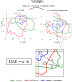
\includegraphics[width=19pc]{schematic.pdf}
\caption{\DIFaddFL{Illustration of the method for calculating the }\textit{\DIFaddFL{difference of absolute errors}} \DIFaddFL{(DAE) in the diurnal signals of an unedited model guidance dataset, and the human edited official forecast dataset, when compared with automatic weather station (AWS) observations, at an example time of 12:00 UTC.}}
\label{Fig:schematic}
\end{figure}
\DIFaddend 

\DIFaddbegin \DIFadd{The first metric I consider is the }\textit{\DIFadd{difference of absolute errors}} \DIFadd{(DAE) in the perturbations, with Fig.~\ref{Fig:schematic} illustrating how DAE is calculated. }\DIFaddend To compare errors in the \DIFdelbegin \DIFdel{official forecast, ACCESS and HRES diurnal cycles we }\DIFdelend \DIFaddbegin \DIFadd{diurnal signals of the official forecast and model guidance, I }\DIFaddend calculate the Euclidean distances between the official or model guidance perturbation vectors at each hour UTC, and the corresponding AWS perturbation vectors at each hour UTC, \DIFaddbegin \DIFadd{and take their difference, }\DIFaddend viewing the Euclidean distance as a measure of absolute error.
\DIFaddbegin 

\DIFaddend For example, to assess whether the official forecast perturbations, \DIFdelbegin \DIFdel{$\boldsymbol{u}_{\text{O}}$, or ACCESS perturbations, $\boldsymbol{u}_{\text{A}}$}\DIFdelend \DIFaddbegin \DIFadd{$\mathbf{u}_{\text{O}}$, or model guidance perturbations, $\mathbf{u}_{\text{M}}$}\DIFaddend , produce lower absolute errors when compared with the observed AWS perturbations, \DIFdelbegin \DIFdel{$\boldsymbol{u}_{\text{AWS}}$, we calculate 
the }\textit{\DIFdel{difference of absolute errors}} %DIFAUXCMD
\DIFdel{(DAE), 
}\DIFdelend \DIFaddbegin \DIFadd{$\mathbf{u}_{\text{AWS}}$, I calculate 
}\DIFaddend \begin{equation}
\text{DAE} \DIFdelbegin \DIFdel{_\text{OA} }\DIFdelend = \left\lvert \DIFdelbegin %DIFDELCMD < \boldsymbol{u}%%%
\DIFdelend \DIFaddbegin \DIFadd{\mathbf{u}}\DIFaddend _{\text{AWS}}-\DIFdelbegin %DIFDELCMD < \boldsymbol{u}%%%
\DIFdel{_{\text{A}} }\DIFdelend \DIFaddbegin \DIFadd{\mathbf{u}_{\text{M}} }\DIFaddend \right\rvert - \left\lvert \DIFdelbegin %DIFDELCMD < \boldsymbol{u}%%%
\DIFdelend \DIFaddbegin \DIFadd{\mathbf{u}}\DIFaddend _{\text{AWS}}-\DIFdelbegin %DIFDELCMD < \boldsymbol{u}%%%
\DIFdelend \DIFaddbegin \DIFadd{\mathbf{u}}\DIFaddend _{\text{O}} \right\rvert. \label{Eq:DAE}
\end{equation} 
\DIFdelbegin \DIFdel{The analogously defined quantities $\text{DAE}_\text{OH}$ and $\text{DAE}_\text{HA}$ provide a comparison of the official forecast and HRES perturbations, and of the HRES and ACCESS perturbations, respectively. We can then take means of the DAE }\DIFdelend \DIFaddbegin \DIFadd{I then calculate statistics from the DAE values }\DIFaddend on an hourly basis\DIFdelbegin \DIFdel{; i.e.~average }\DIFdelend \DIFaddbegin \DIFadd{, in particular, I calculate the arithmetic mean of }\DIFaddend all the 00:00 UTC DAE values, \DIFdelbegin \DIFdel{all the 01:00 UTC values, and so forth, and denote }\DIFdelend \DIFaddbegin \DIFadd{denoting }\DIFaddend such an average by $\overline{\text{DAE}}$\DIFaddbegin \DIFadd{, and repeat this for each hour of the day. If $\overline{\text{DAE}}>0$ at a particular hour, then the official forecast perturbations at that hour are, on average, closer to the observed perturbations than model guidance, and vice versa if $\overline{\text{DAE}}<0$}\DIFaddend .

\DIFdelbegin \DIFdel{Note that $\overline{\text{DAE}}$ compares just }\textit{\DIFdel{one aspect}} %DIFAUXCMD
\DIFdel{of the official forecast with model guidance: it does not, for instance, assess whether the variability of the official forecast is more realistic than that of model guidance. Thus, any statements about performance made throughout this paper refer solely to $\overline{\text{DAE}}$, or subsequently defined metrics, and no claim is being made that these aresufficient to completely characterise the accuracy, or value to the user, of how the diurnal wind cycle is represented in competing forecasts.
}%DIFDELCMD < 

%DIFDELCMD < %%%
\DIFdel{Sea-breeze }\DIFdelend \DIFaddbegin \DIFadd{Diurnal processes like the sea-breeze }\DIFaddend and boundary layer mixing \DIFdelbegin \DIFdel{processes }\DIFdelend depend on the background atmospheric conditions in which they occur. By comparing wind perturbations rather than the overall wind fields \DIFdelbegin \DIFdel{we are }\DIFdelend \DIFaddbegin \DIFadd{I am }\DIFaddend not claiming these background conditions are irrelevant \DIFaddbegin \DIFadd{to these processes}\DIFaddend . However, when a forecaster makes an edit of a wind forecast to better resolve these processes, they are implicitly assuming that future background conditions will be close enough to the preceding 24 hour mean state, or to model predictions of the mean state, to justify making the edit. Thus, it makes sense to compare forecast perturbations to observed perturbations, as long as differences are interpreted as a consequence not only of how the forecaster or model resolves \DIFdelbegin \DIFdel{the diurnal cycle}\DIFdelend \DIFaddbegin \DIFadd{diurnal processes}\DIFaddend , but of how differences in the background state contribute to differences in the perturbations. To minimise the importance of background state differences, this study focuses exclusively on lead-day one forecasts.

Given the large degree of turbulence or random variability in both the AWS, official \DIFaddbegin \DIFadd{forecast}\DIFaddend , and model \DIFaddbegin \DIFadd{guidance }\DIFaddend datasets, care must be taken to \DIFdelbegin \DIFdel{ensure we do not }\DIFdelend \DIFaddbegin \DIFadd{avoid }\DIFaddend pre-emptively \DIFdelbegin \DIFdel{conclude }\DIFdelend \DIFaddbegin \DIFadd{concluding }\DIFaddend the official forecast has outperformed model guidance when $\overline{\text{DAE}}>0$ purely by chance. The method for estimating confidence in $\overline{\text{DAE}}$ is based on a method proposed by \citet{griffiths17}. Time series formed from the DAE values at a particular time, say 00:00 UTC, across the three month time period, are treated as an independent sample of a random variable $E$. The sampling distribution for each $\overline{\text{DAE}}$ can be modelled by a Student's $t$-distribution, and from this \DIFdelbegin \DIFdel{we }\DIFdelend \DIFaddbegin \DIFadd{I }\DIFaddend calculate the probability that $E$ is positive, denoted $\pr\left(E > 0\right)$. 

Although temporal autocorrelations of DAE, i.e.~correlations between DAE values at a particular hour from one day to the next, are in practice small or non-existent, they are still accounted for by reducing the ``effective" sample size to $ n \left(1-\rho_1\right)/\left(1+\rho_1\right)$, where $n$ is the actual sample size and $\rho_1$ is the lag-1 autocorrelation \citep{zwiers95,wilks11}. In the language of statistical hypothesis testing, the null hypothesis that $E=0$ would be rejected at significance level $\alpha$ if $\pr(E>0) > 1-\frac{\alpha}{2}$ or $\pr(E<0) > 1-\frac{\alpha}{2}$. However, in this study \DIFdelbegin \DIFdel{we prefer to }\DIFdelend \DIFaddbegin \DIFadd{I }\DIFaddend simply state the value of $\pr(E>0)$, referring to this as a \textit{confidence score}, and noting $\pr(E<0) = 1- \pr(E>0)$. \DIFdelbegin \DIFdel{We }\DIFdelend \DIFaddbegin \DIFadd{I }\DIFaddend say the official forecast outperforms model guidance with ``high confidence" if $\pr(E>0) \geq 95\%$, or that model guidance outperforms the  official forecast with ``high confidence" if $\pr(E>0) \leq 5\%$, with high confidence implicit whenever it is not explicitly mentioned.

\DIFaddbegin \begin{figure*}
\centering
\includegraphics[width=39pc]{map.pdf}
\caption{\DIFaddFL{Locations of the automatic weather stations, and the groupings of these stations, considered in this study. The }\textit{\DIFaddFL{coastal station groups}} \DIFaddFL{are indicated in a), with the }\textit{\DIFaddFL{airport stations}} \DIFaddFL{shown by stars. The Perth, Adelaide, Melbourne, Hobart, Darwin, Brisbane and Sydney }\textit{\DIFaddFL{city station groups}} \DIFaddFL{are shown shown by b) to h), respectively.}}
\label{Fig:map}
\end{figure*}
\DIFaddend 

Following the ``fuzzy verification" approach outlined by \citet{ebert08}, forecast and observational perturbation datasets are compared not only at individual stations, but are also averaged over two coarser spatial scales before being compared. The individual stations \DIFdelbegin \DIFdel{we }\DIFdelend \DIFaddbegin \DIFadd{I }\DIFaddend consider are the \DIFdelbegin \DIFdel{8 }\DIFdelend \DIFaddbegin \DIFadd{7 }\DIFaddend capital city \textit{airport stations}, marked by stars in Fig.~\ref{Fig:map}, as their high operational significance means that they are typically the most well maintained. An intermediate spatial scale is formed by averaging \DIFaddbegin \DIFadd{perturbation }\DIFaddend data over the 10 stations closest to each capital city airport station, with some flexibility allowed to ensure stations are roughly parallel to the nearest coastline. These station groups are referred to as the \textit{city station groups}. The coarsest spatial scale is formed by averaging over all stations within \DIFdelbegin \DIFdel{150 }\DIFdelend \DIFaddbegin \DIFadd{100 }\DIFaddend km of the nearest coastline, and grouping these by state. The Western Australian coastline \DIFaddbegin \DIFadd{(see Fig.~\ref{Fig:map}) }\DIFaddend is subdivided into three pieces, and stations along the Gulf of Carpentaria, north Queensland Peninsula, and Tasmanian coastlines are neglected, in order to ensure each station group corresponds to an approximately linear segment of coastline to better resolve the land-sea breeze after spatial averaging \citep[e.g.][]{vincent16}. These eight station groups are referred to as the \textit{coastal station groups}.

To compare errors in the perturbations over the two coarser spatial scales, \DIFdelbegin \DIFdel{we }\DIFdelend \DIFaddbegin \DIFadd{I }\DIFaddend modify the definition of DAE in equation (\ref{Eq:DAE}) so that each perturbation dataset is first spatially averaged over either the city or coastal station groups. Confidence scores are calculated for the city and coastal station groups in the same way as for the individual airport stations, treating the spatially averaged data as a single time series. This provides a conservative way to deal with spatial correlation between the stations in each group \citep{griffiths17}. 

To compare biases in the diurnal cycles of each dataset, \DIFdelbegin \DIFdel{we }\DIFdelend \DIFaddbegin \DIFadd{I }\DIFaddend calculate the \textit{difference of biases} (DB),
\begin{equation}
\text{DB} \DIFdelbegin \DIFdel{_{\text{OA}} }\DIFdelend = \left\lvert \DIFdelbegin %DIFDELCMD < \overline{\boldsymbol{u}}%%%
\DIFdelend \DIFaddbegin \overline{\mathbf{u}}\DIFaddend _{\text{AWS}}-\DIFdelbegin %DIFDELCMD < \overline{\boldsymbol{u}}%%%
\DIFdelend \DIFaddbegin \overline{\mathbf{u}}\DIFaddend _{\text{O}} \right\rvert - \left\lvert \DIFdelbegin %DIFDELCMD < \overline{\boldsymbol{u}}%%%
\DIFdelend \DIFaddbegin \overline{\mathbf{u}}\DIFaddend _{\text{AWS}}-\DIFdelbegin %DIFDELCMD < \overline{\boldsymbol{u}}%%%
\DIFdel{_{\text{A}} }\DIFdelend \DIFaddbegin \overline{\mathbf{u}}\DIFadd{_{\text{M}} }\DIFaddend \right\rvert,
\end{equation}
\DIFdelbegin \DIFdel{with $\text{DB}_{\text{OH}}$ and $\text{DB}_{\text{HA}}$ defined analogously, }\DIFdelend where the over-bars denote temporal averages of the perturbations at a particular hour, over June, July and August 2018. These temporally averaged perturbations can be viewed as the \DIFdelbegin \DIFdel{climatological diurnal wind cycles }\DIFdelend \DIFaddbegin \DIFadd{mean diurnal wind cycle }\DIFaddend over the three month study period for each dataset. Biases over the city and coastal station groups are calculated by taking the spatial average before the temporal average. Uncertainty in the DB is estimated through bootstrapping \citep{efron79}. This is done by performing resampling with replacement on the underlying perturbation datasets, and calculating the DB \DIFdelbegin \DIFdel{multiple }\DIFdelend \DIFaddbegin \DIFadd{1000 }\DIFaddend times using these resampled datasets. This provides a distribution of DB values, which analogously to with DAE, \DIFdelbegin \DIFdel{we }\DIFdelend \DIFaddbegin \DIFadd{I }\DIFaddend treat as a sample from a random variable $B$, and use this to estimate $\pr\left(B > 0\right)$.

\DIFaddbegin \DIFadd{Note that on a given day, at a given location, wind perturbations do not necessarily reflect genuinely diurnal processes. There is a large degree of random turbulence in AWS wind observations, and convective cold pools or synoptic fronts can produce rapid changes in background winds that induce large perturbations. However, averaging multiple perturbations at a given hour over many days helps cancel out as much of this non-diurnal variability as possible. When this is repeated for each hour of the day, the signal that remains reflects the mean diurnal cycle (e.g. Figs.~\ref{Fig:darwin_hodo} and \ref{Fig:clim_hodo}). Similar ideas apply to the DAE metric. Note that spatially averaging perturbations accomplishes a similar thing to temporal averaging, helping to cancel out random variability. These ideas can be explored with synthetic data, and some preliminary work to this end is available online \mbox{%DIFAUXCMD
\citep{short20}}\hspace{0pt}%DIFAUXCMD
.
}

\DIFaddend Another approach to forecast verification is to assess structural features of the phenomena being forecast rather than errors or biases of point predictions; this approach is particularly important at small spatiotemporal scales \citep[e.g.][]{mass02, rife05}. \citet{gille05} obtained summary statistics on the observed structure of mean diurnal wind cycles by using linear regression to calculate the coefficients $u_i$, $v_i$ $i=0,1,2$, for the fits 
\begin{align}
u &= u_0 + u_1 \cos(\omega t) + u_2 \sin(\omega t), \label{Eq:u_h} \\
v &= v_0 + v_1 \sin(\omega t) + v_2 \sin(\omega t), \label{Eq:v_h}
\end{align}
where $\omega$ is the angular frequency of the earth and $t$ is the local solar time in seconds. These fits trace out ellipses in the $x,y$ plane, and descriptive metrics like the eccentricity of the ellipse and the angle the semi-major axis makes with lines of latitude, can be calculated directly from the coefficients $u_1$, $u_2$, $v_1$ and $v_2$. \citet{gille05} applied this fit to scatterometer data, which after temporal averaging resulted in just four zonal and meridional values per location, and as such the fit performed very well.  

However, equations (\ref{Eq:u_h}) and (\ref{Eq:v_h}) do not provide a good fit for the hourly data considered here, primarily because they assume a twelve hour symmetry in the evolution of the diurnal cycle. In practice, asymmetries between daytime heating and nighttime cooling \citep[e.g.][]{svensson11} result in surface wind perturbations accelerating rapidly just after sunrise, but remaining comparatively stagnant at night (e.g.~Fig.~\ref{Fig:clim_hodo}). Thus, \DIFdelbegin \DIFdel{we }\DIFdelend \DIFaddbegin \DIFadd{I }\DIFaddend instead fit the equations
\begin{align}
u &= u_0 + u_1 \cos(\alpha(\psi,t)) + u_2 \sin(\alpha(\psi,t)), \label{Eq:u} \\
v &= v_0 + v_1 \sin(\alpha(\psi,t)) + v_2 \sin(\alpha(\psi,t)), \label{Eq:v}
\end{align}
to the climatological perturbations, with $\alpha$ the function from $[0,24) \times [0, 2\pi) \to [0, 2\pi)$ given by
\begin{equation}
\alpha(\psi,t) \equiv \pi \left[\sin\left( \pi \frac{(t - \psi)  \bmod 24}{24} - \frac{\pi}{2} \right) + 1 \right], \label{Eq:alpha}
\end{equation}
with $t$ the time in units of hours UTC, and $\psi$ providing the time when the wind perturbations vary least with time, noting that the same value of $\psi$ is used for both the zonal and meridional perturbations. For each \DIFdelbegin \DIFdel{climatological }\DIFdelend \DIFaddbegin \DIFadd{mean }\DIFaddend diurnal wind cycle, \DIFdelbegin \DIFdel{we }\DIFdelend \DIFaddbegin \DIFadd{I }\DIFaddend solve for the seven parameters $u_0$, $u_1$, $u_2$, $v_0$, $v_1$, $v_2$ and $\psi$ using non-linear regression.

\DIFaddbegin \DIFadd{Importantly, the metrics defined in this section compare just }\textit{\DIFadd{some aspects}} \DIFadd{of the official forecast with model guidance: they do not, for instance, assess whether diurnal variance of the official forecast is more realistic than that of model guidance. Thus, any statements about performance made throughout this paper refer solely to the metrics defined here, and }\textit{\DIFadd{no claim}} \DIFadd{is being made that these are sufficient to completely characterise the accuracy, or value to the user, of how the diurnal wind cycle is represented in competing forecasts. Furthermore, comparing results at different locations is }\textit{\DIFadd{not}} \DIFadd{intended as a ``ranking" of forecasting centres in different states because, for instance, station density varies significantly with location so it is hard to define station groups at a given spatial scale in a completely consistent way across locations. Such issues are a fundamental limitation of station based verification.
}\DIFaddend 

\section{Results}
\label{Sec:Results}
In this section, the methods described in section \ref{Sec:Methods} are applied to Australian forecast and station data over the months of June, July and August 2018. First, \DIFaddbegin \DIFadd{mean }\DIFaddend differences in absolute errors (DAE) and differences in biases (DB) over this time period are assessed. Second, structural indices are compared to elucidate the physical reasons for biases. \DIFaddbegin \DIFadd{Unless otherwise noted, times are given in UTC.
}\DIFaddend 

\begin{figure*}
\centering
 %DIFDELCMD < 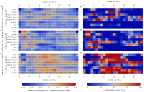
\includegraphics[width=39pc]{old_figures/wpi_coastal.pdf}
%DIFDELCMD < %%%
\includegraphics[width=39pc]{coastal_DAE.pdf}
\caption{Heatmaps of mean difference of absolute error $\overline{\text{DAE}}$ values, a), c), e), and confidence scores, b), d), f), for \DIFdelbeginFL \DIFdelFL{each coastal station group }\DIFdelendFL \DIFaddbeginFL \DIFaddFL{the }\textit{\DIFaddFL{coastal station groups}} \DIFaddendFL (see Fig.~\ref{Fig:map})\DIFdelbeginFL \DIFdelFL{and }\DIFdelendFL \DIFaddbeginFL \DIFaddFL{. Results given for each }\DIFaddendFL hour of the day, for the official forecast versus ACCESS, a) and b), official forecast versus HRES, c) and d), \DIFdelbeginFL \DIFdelFL{HRES }\DIFdelendFL \DIFaddbeginFL \DIFaddFL{and official forecast }\DIFaddendFL versus \DIFdelbeginFL \DIFdelFL{ACCESS}\DIFdelendFL \DIFaddbeginFL \DIFaddFL{OCF}\DIFaddendFL , e) and f)\DIFaddbeginFL \DIFaddFL{, comparisons}\DIFaddendFL . Positive $\overline{\text{DAE}}$ values indicate that the former dataset in each pair is on average $\overline{\text{DAE}}$ \DIFdelbeginFL \DIFdelFL{kn }\DIFdelendFL \DIFaddbeginFL \DIFaddFL{kt }\DIFaddendFL closer to observations than the latter dataset (see equation \ref{Eq:DAE}), where $1$ \DIFdelbeginFL \DIFdelFL{kn }\DIFdelendFL \DIFaddbeginFL \DIFaddFL{kt }\DIFaddendFL $\approx 0.514$ m s\textsuperscript{-1}. Confidence scores provide the probability the population or ``true" value of $\overline{\text{DAE}}$ is greater than zero (see section \ref{Sec:Methods}).}
\label{Fig:coastal_DAE}
\end{figure*}

\begin{figure}
\centering
 %DIFDELCMD < \includegraphics[width=19pc]{old_figures/case_studies_nt.pdf}
%DIFDELCMD < %%%
 \includegraphics[width=19pc]{case_studies_nt.pdf}
\caption{Time series, a), of the difference in absolute error DAE defined in equation (\ref{Eq:DAE}) for the official forecast versus ACCESS, \DIFdelbeginFL \DIFdelFL{$\text{DAE}_\text{OA}$, and }\DIFdelendFL official forecast versus HRES, \DIFdelbeginFL \DIFdelFL{$\text{DAE}_\text{OH}$}\DIFdelendFL \DIFaddbeginFL \DIFaddFL{and official forecast versus OCF comparisons}\DIFaddendFL , for the \DIFaddbeginFL \DIFaddFL{Northern Territory (}\DIFaddendFL NT\DIFaddbeginFL \DIFaddFL{) }\DIFaddendFL coastal station group shown in Fig.~\ref{Fig:map}\DIFaddbeginFL \DIFaddFL{, }\DIFaddendFL at 23:00 UTC. Also, temporal hodographs in hours UTC showing hourly changes in winds, b), and wind perturbations from a 24 hour running mean, c), at the NT coastal station group on the 3\textsuperscript{rd} of July 2018.}
\label{Fig:case_studies_nt}
\end{figure}

\subsection{Absolute Errors}
\label{Sec:Daily}

Figure \DIFdelbegin \DIFdel{\ref{Fig:wpi_coastal} }\DIFdelend \DIFaddbegin \DIFadd{\ref{Fig:coastal_DAE} }\DIFaddend provides the mean difference of absolute error \DIFdelbegin \DIFdel{$\overline{\text{DAE}}$ }\DIFdelend values and confidence scores defined in section \ref{Sec:Methods} for the coastal station groups shown in Fig.~\ref{Fig:map}\DIFdelbegin \DIFdel{, for $\overline{\text{DAE}}_\text{OA}$, $\overline{\text{DAE}}_\text{OH}$ and $\overline{\text{DAE}}_\text{HA}$, which represent }\DIFdelend \DIFaddbegin \DIFadd{. Results are given for }\DIFaddend the official forecast versus ACCESS, official forecast versus HRES, and \DIFdelbegin \DIFdel{HRES versus ACCESS comparisons, respectively}\DIFdelend \DIFaddbegin \DIFadd{official forecast versus OCF comparisons}\DIFaddend . The results indicate that for the majority of station groups and hours, \DIFdelbegin \DIFdel{both }\DIFdelend the unedited ACCESS\DIFdelbegin \DIFdel{and HRES models }\DIFdelend \DIFaddbegin \DIFadd{, HRES and OCF datasets }\DIFaddend outperform the official forecast. The lowest $\overline{\text{DAE}}$ values occur at the \DIFdelbegin \DIFdel{NT }\DIFdelend \DIFaddbegin \DIFadd{Northern Territory (NT) }\DIFaddend station group at 23:00 and 00:00 \DIFdelbegin \DIFdel{UTC for both $\overline{\text{DAE}}_\text{OA}$ and $\overline{\text{DAE}}_\text{OH}$}\DIFdelend \DIFaddbegin \DIFadd{for both the official forecast versus ACCESS, and official forecast versus HRES comparisons, and at 22:00 and 23:00 for the official forecast versus OCF comparison}\DIFaddend . Although the official forecast outperforms at least one of ACCESS\DIFdelbegin \DIFdel{or HRES }\DIFdelend \DIFaddbegin \DIFadd{, HRES and OCF }\DIFaddend at multiple times and station groups, the only group and time where it outperforms \DIFdelbegin \DIFdel{both }\DIFdelend \DIFaddbegin \DIFadd{all three }\DIFaddend is 05:00 UTC over the South \DIFdelbegin \DIFdel{WA }\DIFdelend \DIFaddbegin \DIFadd{Western Australia (WA) }\DIFaddend station group.
\DIFdelbegin \DIFdel{HRES generally outperforms ACCESS from 10:00 - 14:00 UTC, with the South WA station group being the main exception.    
}\DIFdelend 

Figures \ref{Fig:case_studies_nt} and \ref{Fig:case_studies_wa} provide case studies of the \DIFdelbegin \DIFdel{NT and South WA }\DIFdelend \DIFaddbegin \DIFadd{Northern Territory (NT) and South Western Australia (WA) }\DIFaddend station groups, respectively. Figure \ref{Fig:case_studies_nt} a) provides a time series of DAE for the NT station group at 23:\DIFdelbegin \DIFdel{00 UTC. }\DIFdelend \DIFaddbegin \DIFadd{00. }\DIFaddend The time series shows significant temporal variability, with DAE frequently dropping below $-2$ \DIFdelbegin \DIFdel{kn}\DIFdelend \DIFaddbegin \DIFadd{kt}\DIFaddend . Figures \ref{Fig:case_studies_nt} b) and c) show hodographs of the winds and wind perturbations, respectively, at each hour UTC on the 3\textsuperscript{rd} of July, which provides an interesting example. \DIFaddbegin \DIFadd{Note that care must be taken when interpreting DAE scores on individual days physically, as discussed in section \ref{Sec:Methods}. 
}\DIFaddend 

Figure \ref{Fig:case_studies_nt} b) shows that the official wind forecast on this day was likely based on edited ACCESS from 00:00 to 06:00\DIFdelbegin \DIFdel{UTC}\DIFdelend , then edited HRES from 07:00 to 13:00 UTC, then unedited ACCESS from 15:00 to 21:\DIFdelbegin \DIFdel{00 UTC. }\DIFdelend \DIFaddbegin \DIFadd{00. }\DIFaddend At 22:00 and 23:00\DIFdelbegin \DIFdel{UTC}\DIFdelend , the official forecast winds acquire stronger \DIFdelbegin \DIFdel{east-northeasterly }\DIFdelend \DIFaddbegin \DIFadd{east-southeasterly }\DIFaddend components than the other datasets. \DIFdelbegin \DIFdel{Figure \ref{Fig:perth_sounding} }\DIFdelend \DIFaddbegin \DIFadd{For comparison, Fig.~\ref{Fig:soundings} }\DIFaddend a) shows the first ten values from wind soundings at Darwin Airport at 12:00 \DIFdelbegin \DIFdel{UTC }\DIFdelend on July 3\textsuperscript{rd} and 00:00 \DIFdelbegin \DIFdel{UTC }\DIFdelend on July 4\textsuperscript{th}. In both instances the winds are east-southeasterly, and so the rapidly changing wind perturbations at 22:00 \DIFdelbegin \DIFdel{UTC }\DIFdelend in the official forecast \DIFdelbegin \DIFdel{likely }\DIFdelend \DIFaddbegin \DIFadd{may }\DIFaddend reflect a boundary layer mixing edit that has been applied either too early, or has strengthened the southeasterly component of the winds too much. Similar issues \DIFdelbegin \DIFdel{create }\DIFdelend \DIFaddbegin \DIFadd{appear to create the }\DIFaddend low DAE values on the 8\textsuperscript{th} of June and 9\textsuperscript{th} and 10\textsuperscript{th} of July.

Figure \ref{Fig:case_studies_wa} a) provides a time series of DAE for the South WA station group at 05:\DIFdelbegin \DIFdel{00 UTC. }\DIFdelend \DIFaddbegin \DIFadd{00. }\DIFaddend As with the NT station group there is significant temporal variability, with DAE frequently exceeding 1 \DIFdelbegin \DIFdel{kn}\DIFdelend \DIFaddbegin \DIFadd{kt}\DIFaddend . Figures \ref{Fig:case_studies_wa} b) and c) provide hodographs of the winds and wind perturbations, respectively, on the 9\textsuperscript{th} of June, another interesting example. \DIFdelbegin \DIFdel{The perturbation hodograph shows }\DIFdelend \DIFaddbegin \DIFadd{Both the raw winds and the perturbations appear to show }\DIFaddend both HRES and ACCESS under-predicting the amplitude of the diurnal wind cycle on this day\DIFdelbegin \DIFdel{. Figure \ref{Fig:perth_sounding} }\DIFdelend \DIFaddbegin \DIFadd{, with OCF performing better in this regard. Figure \ref{Fig:soundings} b) }\DIFaddend shows wind soundings at Perth Airport, the nearest station to provide wind soundings, between 12:00 \DIFdelbegin \DIFdel{UTC }\DIFdelend on the 8\textsuperscript{th} June and 12:00 \DIFdelbegin \DIFdel{UTC }\DIFdelend on the 9\textsuperscript{th} June. The 8\textsuperscript{th} June 12:00 \DIFdelbegin \DIFdel{UTC }\DIFdelend sounding shows surface northerlies of around $6$ \DIFdelbegin \DIFdel{kn}\DIFdelend \DIFaddbegin \DIFadd{kt}\DIFaddend , becoming west to northwesterlies of over 20 \DIFdelbegin \DIFdel{kn }\DIFdelend \DIFaddbegin \DIFadd{kt }\DIFaddend $2.4$ km above the surface. However, the subsequent sounding at 00:00 \DIFdelbegin \DIFdel{UTC }\DIFdelend on the 9\textsuperscript{th} of June shows that the winds acquire a strong northerly component of 30 \DIFdelbegin \DIFdel{kn }\DIFdelend \DIFaddbegin \DIFadd{kt }\DIFaddend in the first 500 m of the atmosphere, with the final sounding indicating a strong northwesterly wind at 725 m persisting until 12:\DIFdelbegin \DIFdel{00 UTC. 
}\DIFdelend \DIFaddbegin \DIFadd{00. 
}\DIFaddend 

In Fig.~\ref{Fig:case_studies_wa} c), the \DIFaddbegin \DIFadd{OCF and }\DIFaddend official forecast perturbations from 04:00 to 07:00 \DIFdelbegin \DIFdel{UTC }\DIFdelend show stronger westerly perturbations than either ACCESS or HRES, improving the \DIFdelbegin \DIFdel{amplitude of the official forecast's diurnal wind cycle}\DIFdelend \DIFaddbegin \DIFadd{magnitude of both dataset's perturbations}\DIFaddend . However, the AWS perturbations are more northerly than those of the official forecast \DIFdelbegin \DIFdel{, and so the official forecast winds have been strengthened in a slightly incorrect direction. One explanation }\DIFdelend \DIFaddbegin \DIFadd{or OCF. Possible explanations }\DIFaddend for this discrepancy \DIFdelbegin \DIFdel{is }\DIFdelend \DIFaddbegin \DIFadd{are }\DIFaddend that the official forecast has been edited based on the June 8\textsuperscript{th} 12:00 \DIFdelbegin \DIFdel{UTC }\DIFdelend sounding, with the winds above the surface changing direction in the subsequent 12 hours\DIFdelbegin \DIFdel{. A similar explanation can be given for the high DAE scores on the  3\textsuperscript{rd} of August, although in this case }\DIFdelend \DIFaddbegin \DIFadd{, or that }\DIFaddend the official forecast \DIFdelbegin \DIFdel{slightly improves both the magnitude and direction of the 05:00 UTC wind }\DIFdelend \DIFaddbegin \DIFadd{has been based on OCF, which underestimates the northerly component of the }\DIFaddend perturbations.

\begin{figure}
\centering
%DIFDELCMD < \includegraphics[width=19pc]{old_figures/case_studies_wa.pdf}
%DIFDELCMD < %%%
\includegraphics[width=19pc]{case_studies_wa.pdf}
\caption{As in Fig.~\ref{Fig:case_studies_nt}, but for, a), the South \DIFaddbeginFL \DIFaddFL{Western Australia (}\DIFaddendFL WA\DIFaddbeginFL \DIFaddFL{) }\DIFaddendFL coastal station group at 05:00 UTC, and b) and c), the winds and wind perturbations, respectively, over the South WA coastal station group on the 9\textsuperscript{th} June 2018.} 
\label{Fig:case_studies_wa}
\end{figure}

\begin{figure*}
\centering
%DIFDELCMD < 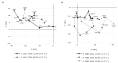
\includegraphics[width=33pc]{old_figures/perth_sounding.pdf}
%DIFDELCMD < %%%
\includegraphics[width=33pc]{soundings.pdf}
\caption{Vertical wind soundings at, a), Darwin Airport, and b), Perth Airport, with heights given in metres.}
 %DIFDELCMD < \label{Fig:perth_sounding}
%DIFDELCMD < %%%
\label{Fig:soundings}
 \end{figure*}

\begin{figure*}
\centering
 %DIFDELCMD < 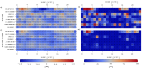
\includegraphics[width=39pc]{old_figures/airport_wpi.pdf}
%DIFDELCMD < %%%
\includegraphics[width=39pc]{city_DAE.pdf}
\caption{As in Fig.~\DIFdelbeginFL \DIFdelFL{\ref{Fig:wpi_coastal}}\DIFdelendFL \DIFaddbeginFL \DIFaddFL{\ref{Fig:coastal_DAE}}\DIFaddendFL , but for the official \DIFaddbeginFL \DIFaddFL{forecast }\DIFaddendFL versus HRES \DIFdelbeginFL \DIFdelFL{mean difference of absolute error $\overline{\text{DAE}}_\text{OH}$ values, }\DIFdelendFL \DIFaddbeginFL \DIFaddFL{comparison }\DIFaddendFL a) and \DIFdelbeginFL \DIFdelFL{c}\DIFdelendFL \DIFaddbeginFL \DIFaddFL{b}\DIFaddendFL ), and \DIFdelbeginFL \DIFdelFL{confidence scores}\DIFdelendFL \DIFaddbeginFL \DIFaddFL{the official forecast versus OCF comparison}\DIFaddendFL , \DIFdelbeginFL \DIFdelFL{b}\DIFdelendFL \DIFaddbeginFL \DIFaddFL{c}\DIFaddendFL ) and d), for the \DIFdelbeginFL \DIFdelFL{airport stations, a) and b), and city station groups, c) and d)}\DIFdelendFL \DIFaddbeginFL \textit{\DIFaddFL{city station groups}} \DIFaddFL{(see Fig}\DIFaddendFL .\DIFaddbeginFL \DIFaddFL{~\ref{Fig:map}.)}\DIFaddendFL }
 %DIFDELCMD < \label{Fig:airport_wpi}
%DIFDELCMD < %%%
\DIFdelendFL \label{Fig:city_DAE}
\end{figure*}

\begin{figure*}
\centering
\includegraphics[width=39pc]{airport_DAE.pdf}
\caption{\DIFaddFL{As in Fig.~\ref{Fig:coastal_DAE}, but for the official forecast versus HRES comparison a) and b), and the official forecast versus OCF comparison, c) and d), for the }\textit{\DIFaddFL{airport stations}} \DIFaddFL{(see Fig.~\ref{Fig:map}.)}}
\label{Fig:airport_DAE}
\end{figure*}

Fig.~\DIFdelbegin \DIFdel{\ref{Fig:airport_wpi} }\DIFdelend \DIFaddbegin \DIFadd{\ref{Fig:city_DAE} }\DIFaddend presents the $\overline{\text{DAE}}$ values and confidence scores for the \DIFdelbegin \DIFdel{airport stations, and }\DIFdelend city station groups, for the official forecast versus HRES \DIFdelbegin \DIFdel{comparison, i.e.~$\overline{\text{DAE}}_\text{OH}$. The results for the airport stations are noisier than the results for the coastal station groups in Figs.~\ref{Fig:wpi_coastal} c) and d), although they share some similarities. For instance, the official forecast outperforms HRES at 01:00 }\DIFdelend and \DIFdelbegin \DIFdel{02:00 UTC at both the Darwin airport station and the NT coastal station group. There are four other instances where }\DIFdelend \DIFaddbegin \DIFadd{official forecast versus OCF comparisons; }\DIFaddend the official forecast \DIFdelbegin \DIFdel{outperforms HRES with at least $90\%$ confidence, although this could simply be occurring by chance due repeated testing \mbox{%DIFAUXCMD
\citep[p. 178]{wilks11}}\hspace{0pt}%DIFAUXCMD
. }%DIFDELCMD < 

%DIFDELCMD < %%%
\DIFdel{For the city station groups, HRES outperforms }\DIFdelend \DIFaddbegin \DIFadd{versus ACCESS comparisons (not shown) are similar to those for HRES and have been omitted for space. Both HRES and OCF outperform }\DIFaddend the official forecast almost uniformly\DIFdelbegin \DIFdel{. The main exception is }\DIFdelend \DIFaddbegin \DIFadd{, with }\DIFaddend the Darwin city station group \DIFdelbegin \DIFdel{, where }\DIFdelend \DIFaddbegin \DIFadd{the main exception. At Darwin, }\DIFaddend the official forecast outperforms \DIFdelbegin \DIFdel{HRES }\DIFdelend \DIFaddbegin \DIFadd{both HRES and OCF }\DIFaddend at 02:00 UTC, and there is ambiguity \DIFdelbegin \DIFdel{as to whether the official forecast or HRES performs better at 01:00, 03:00 and 04:00 UTC, and from 15:00 to 22:00 UTC. The analogous $\overline{\text{DAE}}_\text{OA}$ official forecast versus ACCESS comparisons (not shown) are similar, with the airport station results noisy, but ACCESS outperforming the official forecast over the city station groups for the vast majority of times and locations. Over the }\DIFdelend \DIFaddbegin \DIFadd{at some other times of day. The OCF comparison shows less ambiguity at Darwin, but more at Melbourne and Brisbane. The city station group results for }\DIFaddend December, January, February 2017/18 \DIFdelbegin \DIFdel{season, HRES also outperforms the official forecast almost uniformly over the city station groups, although the official forecast versus ACCESS comparisons are more ambiguous. 
}%DIFDELCMD < 

%DIFDELCMD < \begin{figure*}
%DIFDELCMD < \centering
%DIFDELCMD < 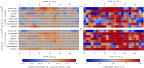
\includegraphics[width=39pc]{old_figures/airport_wpi_EA.pdf}
%DIFDELCMD < %%%
%DIFDELCMD < \caption{%
{%DIFAUXCMD
\DIFdelFL{As in Fig.~\ref{Fig:airport_wpi}, but for the HRES versus ACCESS mean difference in absolute error $\overline{\text{DAE}}_\text{HA}$ values and confidence scores.
}}
%DIFAUXCMD
%DIFDELCMD < \label{Fig:airport_wpi_EA}
%DIFDELCMD < \end{figure*}
%DIFDELCMD < 

%DIFDELCMD < %%%
\DIFdel{Figure \ref{Fig:airport_wpi_EA} provides the $\overline{\text{DAE}}$ values and confidence scores for the airport stations, and }\DIFdelend \DIFaddbegin \DIFadd{(not shown) are similar but slightly more ambiguous, particularly for ACCESS. These results were replicated using alternative }\DIFaddend city station groups, \DIFdelbegin \DIFdel{for the HRES versus ACCESS comparison.
As with }\DIFdelend \DIFaddbegin \DIFadd{defined by taking all stations within 100 km $\times$ 100 km boxes centred on each capital city airport: the results (not shown) were very similar, with both HRES and OCF almost uniformly outperforming the official forecast.
}

\DIFaddend Fig.~\DIFdelbegin \DIFdel{\ref{Fig:airport_wpi}, the results }\DIFdelend \DIFaddbegin \DIFadd{\ref{Fig:airport_DAE} presents the comparisons }\DIFaddend for the airport stations\DIFdelbegin \DIFdel{are noisy, but more often than not show that HRES outperforms ACCESS. The results for the city station groups show HRES usually outperforms ACCESS, the main exceptions being the Darwin and Canberra city station groups. Results for the December, January, February 2017/18 season are again similar, but here HRES outperforms ACCESS over the city station groups almost uniformly}\DIFdelend \DIFaddbegin \DIFadd{. Here the results are noisier than at both the city and coastal spatial scales, but similarities also exist. For instance, the official forecast outperforms both OCF and HRES at 02:00 at Darwin airport, the Darwin city station group, and the NT coastal station group with at least $90\%$ confidence. There are four other instances where the official forecast outperforms HRES with at least $90\%$ confidence, although this could simply be occurring by chance due repeated testing \mbox{%DIFAUXCMD
\citep[p. 178]{wilks11}}\hspace{0pt}%DIFAUXCMD
. By contrast, the official forecast outperforms OCF over four hour intervals at both Perth and Brisbane airports}\DIFaddend .

\subsection{Seasonal Biases}
\label{Sec:Seasonal}
Figure \DIFdelbegin \DIFdel{\ref{Fig:cwpi_coastal} }\DIFdelend \DIFaddbegin \DIFadd{\ref{Fig:DB_coastal} }\DIFaddend provides the difference of biases (DB) and confidence scores defined in section \ref{Sec:Methods}, for the coastal station groups\DIFdelbegin \DIFdel{for $\text{DB}_\text{OA}$}\DIFdelend , \DIFdelbegin \DIFdel{$\text{DB}_\text{OH}$ and $\text{DB}_\text{HA}$, which represent the }\DIFdelend \DIFaddbegin \DIFadd{for }\DIFaddend the official forecast versus ACCESS, official forecast versus HRES, and \DIFdelbegin \DIFdel{HRES versus ACCESS comparisons, respectively}\DIFdelend \DIFaddbegin \DIFadd{official forecast versus OCF comparisons}\DIFaddend . At the NT station \DIFaddbegin \DIFadd{group }\DIFaddend at 03:00\DIFdelbegin \DIFdel{UTC}\DIFdelend , the official forecast outperforms both ACCESS and HRES with confidence $\geq 93\%$. However, \DIFdelbegin \DIFdel{both ACCESSand HRES }\DIFdelend \DIFaddbegin \DIFadd{ACCESS, HRES and OCF each }\DIFaddend outperform the official forecast at 23:00 and 00:00\DIFdelbegin \DIFdel{UTC}\DIFdelend , and from \DIFdelbegin \DIFdel{05}\DIFdelend \DIFaddbegin \DIFadd{06}\DIFaddend :00 to \DIFdelbegin \DIFdel{11}\DIFdelend \DIFaddbegin \DIFadd{10}\DIFaddend :00\DIFdelbegin \DIFdel{UTC}\DIFdelend , consistent with the $\overline{\text{DAE}}$ results of Fig.~\DIFdelbegin \DIFdel{\ref{Fig:wpi_coastal}. Figure \ref{Fig:clim_hodo} a}\DIFdelend \DIFaddbegin \DIFadd{\ref{Fig:coastal_DAE}. Figure \ref{Fig:darwin_hodo} c}\DIFaddend ) shows that these \DIFdelbegin \DIFdel{biases are mostly a consequence of }\DIFdelend \DIFaddbegin \DIFadd{DB results reflect }\DIFaddend amplitude biases in the official forecast's \DIFaddbegin \DIFadd{mean }\DIFaddend diurnal cycle.

\begin{figure*}
\centering
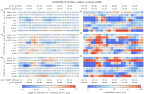
\includegraphics[width=39pc]{DB_coastal.pdf}
\caption{\DIFaddFL{As in Fig.~\ref{Fig:coastal_DAE}, but for the difference of biases (DB) values and confidence scores.}}
\label{Fig:DB_coastal}
\end{figure*}

\begin{figure*}
\centering
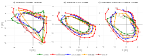
\includegraphics[width=39pc]{darwin_hodo.pdf}
\caption{\DIFaddFL{Temporal hodographs in hours UTC of wind perturbations at, a), Darwin Airport, b), spatially averaged over the Darwin city station group, and c), the NT coastal group (see Fig.~\ref{Fig:map}), then temporally averaged over June, July and August 2018.}}
\label{Fig:darwin_hodo}
\end{figure*}

\DIFaddend At the South WA station group from 01:00 to 05:00\DIFdelbegin \DIFdel{UTC}\DIFdelend , the official forecast outperforms HRES with confidence scores of at least $88\%$. Figure \ref{Fig:clim_hodo} \DIFdelbegin \DIFdel{b}\DIFdelend \DIFaddbegin \DIFadd{a}\DIFaddend ) shows that HRES underestimates the westerly perturbations at these times, with these perturbations \DIFdelbegin \DIFdel{likely }\DIFdelend \DIFaddbegin \DIFadd{potentially }\DIFaddend associated with boundary layer mixing processes, as discussed in section \ref{Sec:Results} \ref{Sec:Daily}. \DIFdelbegin \DIFdel{Each of the }\DIFdelend \DIFaddbegin \DIFadd{The }\DIFaddend official forecast, ACCESS and HRES \DIFaddbegin \DIFadd{all }\DIFaddend underestimate the amplitude of the diurnal cycle between 02:00 and 10:00\DIFdelbegin \DIFdel{UTC}\DIFdelend , including both the westerly perturbations and the southerly sea-breeze perturbations. \DIFdelbegin %DIFDELCMD < 

%DIFDELCMD < %%%
\DIFdel{At the NSW station group from 17}\DIFdelend \DIFaddbegin \DIFadd{OCF better approximates the amplitude of the diurnal cycle between 02}\DIFaddend :00 \DIFdelbegin \DIFdel{to 19}\DIFdelend \DIFaddbegin \DIFadd{and 05}\DIFaddend :00\DIFdelbegin \DIFdel{UTC, the official forecast outperforms both ACCESS and HRES with confidence scores of at least least 95\% and 75\%, respectively. Figure \ref{Fig:clim_hodo} c) shows that these times correspond to ``dimples" in the perturbation temporal hodographs that are present in all four datasets. The official forecast hodograph closely resembles that of ACCESS, except for this dimple, which has been exaggerated relative to ACCESS. Figure \ref{Fig:clim_hodo} c) also shows that although HRES exaggerates the amplitude of the easterly sea-breeze perturbations , it captures the narrower shape of the AWS hodograph better than the official forecast or ACCESS.
}\DIFdelend \DIFaddbegin \DIFadd{, but shows the greatest underestimation of the southerly perturbations between 06:00 and 10:00.
}\DIFaddend 

At the \DIFdelbegin \DIFdel{SA station group }\DIFdelend \DIFaddbegin \DIFadd{South Australia (SA) station group, the official forecast slightly outperforms ACCESS and HRES }\DIFaddend from 02:00 to 05:00 \DIFdelbegin \DIFdel{UTC }\DIFdelend and 09:00 to 12:00\DIFdelbegin \DIFdel{UTC, the official forecast outperforms both ACCESS and HRES}\DIFdelend \DIFaddbegin \DIFadd{, although confidence scores do not exceed 64\% and 90\% respectively. The official forecast also slightly outperforms OCF between 00:00 and 02:00, and between 08:00 and 09:00}\DIFaddend , although confidence scores do not exceed \DIFdelbegin \DIFdel{88\% and 65\%respectively}\DIFdelend \DIFaddbegin \DIFadd{74\%}\DIFaddend . Figure \ref{Fig:clim_hodo} \DIFdelbegin \DIFdel{d}\DIFdelend \DIFaddbegin \DIFadd{b}\DIFaddend ) shows that although the official forecast captures the amplitude of the perturbations from 01:00 to 05:00 \DIFdelbegin \DIFdel{UTC }\DIFdelend almost perfectly, its \DIFaddbegin \DIFadd{mean }\DIFaddend diurnal cycle is out of phase with that of \DIFdelbegin \DIFdel{the }\DIFdelend AWS during this period, explaining \DIFdelbegin \DIFdel{why the official forecast only slightly outperforms ACCESS in the results of Figures \ref{Fig:cwpi_coastal} a) and b)}\DIFdelend \DIFaddbegin \DIFadd{the only slightly positive DB values}\DIFaddend .

 %DIFDELCMD < \begin{figure*}
%DIFDELCMD < \centering
%DIFDELCMD < 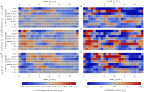
\includegraphics[width=39pc]{old_figures/cwpi_coastal.pdf}
%DIFDELCMD < %%%
%DIFDELCMD < \caption{%
{%DIFAUXCMD
\DIFdelFL{As in Fig.~\ref{Fig:wpi_coastal}, but for the difference of biases (DB) values and confidence scores.}}
%DIFAUXCMD
%DIFDELCMD < \label{Fig:cwpi_coastal}
%DIFDELCMD < \end{figure*}
%DIFDELCMD < 

%DIFDELCMD < \begin{figure*}
%DIFDELCMD < %%%
\begin{figure}
\centering
 %DIFDELCMD < 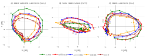
\includegraphics[width=33pc]{old_figures/clim_hodo_alt.pdf}
%DIFDELCMD < %%%
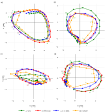
\includegraphics[width=19pc]{clim_hodo.pdf}
\caption{Temporal hodographs in hours UTC of \DIFaddbeginFL \DIFaddFL{diurnal }\DIFaddendFL wind perturbations spatially averaged over the, a), \DIFdelbeginFL \DIFdelFL{NT, b) }\DIFdelendFL South \DIFaddbeginFL \DIFaddFL{Western Australia (}\DIFaddendFL WA\DIFdelbeginFL \DIFdelFL{, c}\DIFdelendFL )\DIFdelbeginFL \DIFdelFL{NSW }\DIFdelendFL \DIFaddbeginFL \DIFaddFL{, }\DIFaddendFL and \DIFdelbeginFL \DIFdelFL{d}\DIFdelendFL \DIFaddbeginFL \DIFaddFL{b}\DIFaddendFL ), \DIFaddbeginFL \DIFaddFL{South Australia (}\DIFaddendFL SA\DIFaddbeginFL \DIFaddFL{) }\DIFaddendFL coastal station groups (see Fig.~\ref{Fig:map}), and temporally averaged over June, July and August 2018.}
\label{Fig:clim_hodo}
%DIFDELCMD < \end{figure*}
%DIFDELCMD < 

%DIFDELCMD < \begin{figure*}
%DIFDELCMD < \centering
%DIFDELCMD < 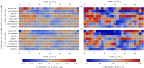
\includegraphics[width=39pc]{old_figures/airport_cwpi.pdf}
%DIFDELCMD < %%%
%DIFDELCMD < \caption{%
{%DIFAUXCMD
\DIFdelFL{As in Fig.~\ref{Fig:airport_wpi}, but for the difference of biases (DB) values and confidence scores.}}
%DIFAUXCMD
%DIFDELCMD < \label{Fig:airport_cwpi}
%DIFDELCMD < \end{figure*}
%DIFDELCMD < %%%
\end{figure}

For comparison, \DIFdelbegin \DIFdel{Fig.~\ref{Fig:airport_cwpi} presents }\DIFdelend \DIFaddbegin \DIFadd{Figs.~\ref{Fig:DB_city} and \ref{Fig:DB_airport} present }\DIFaddend the DB values and confidence scores for \DIFdelbegin \DIFdel{$\text{DB}_\text{OH}$, which represents }\DIFdelend the official forecast versus HRES \DIFdelbegin \DIFdel{comparison}\DIFdelend \DIFaddbegin \DIFadd{and official forecast versus OCF comparisons}\DIFaddend , for the \DIFdelbegin \DIFdel{airport stations and }\DIFdelend city station groups \DIFaddbegin \DIFadd{and airport stations, respectively}\DIFaddend . Some regions exhibit consistent results across all three spatial scales\DIFdelbegin \DIFdel{, for }\DIFdelend \DIFaddbegin \DIFadd{. For }\DIFaddend example, the official forecast \DIFdelbegin \DIFdel{is less biased than HRES }\DIFdelend \DIFaddbegin \DIFadd{outperforms HRES between 14:00 and 18:00, }\DIFaddend with at least \DIFdelbegin \DIFdel{$80 \%$ confidence}\DIFdelend \DIFaddbegin \DIFadd{$83\%$ confidence, }\DIFaddend at Sydney airport, the Sydney city station group, and the NSW coastal station group\DIFdelbegin \DIFdel{, from 14:00 to 18:00 UTC}\DIFdelend . 

\DIFaddbegin \DIFadd{Other results are markedly different between spatial scales. For instance, the official forecast outperforms OCF for most of the day at Darwin airport, but the opposite is true at the Darwin city and NT coastal station groups. Figure \ref{Fig:darwin_hodo} a) shows that the mean AWS diurnal cycle is highly asymmetric, with a sharp peak occurring at 06:00. This peak is captured well by HRES and the official forecast, but not by OCF or ACCESS. Figures \ref{Fig:darwin_hodo} b) and c) show that over the Darwin city and NT coastal station groups, the mean diurnal cycles are much smoother, with the amplitudes of the official forecast diurnal cycles exaggerated relative to AWS and OCF. 
}

\begin{figure*}
\centering
\includegraphics[width=39pc]{DB_city.pdf}
\caption{\DIFaddFL{As in Fig.~\ref{Fig:city_DAE}, but for the difference of biases (DB) values and confidence scores.}}
\label{Fig:DB_city}
\end{figure*}

\begin{figure*}
\centering
\includegraphics[width=39pc]{DB_airport.pdf}
\caption{\DIFaddFL{As in Fig.~\ref{Fig:airport_DAE}, but for the difference of biases (DB) values and confidence scores.}}
\label{Fig:DB_airport}
\end{figure*}

\DIFaddend \subsection{Ellipse Fits}

\begin{figure}
\centering
\DIFdelbeginFL %DIFDELCMD < \includegraphics[width=19pc]{old_figures/r_squared.pdf}
%DIFDELCMD < %%%
\DIFdelendFL \DIFaddbeginFL \includegraphics[width=19pc]{r_squared.pdf}
\DIFaddendFL \caption{$R^2$ values as percentages for the fit of equation (\ref{Eq:u}) to the zonal perturbations, a), c) and e), and equation (\ref{Eq:v}) to the meridional perturbations, b), d) and f), for the airport stations, a) and b), city station groups, c) and d), and coastal station groups, e) and f), shown in Fig.~\ref{Fig:map}.}
\label{Fig:r_squared}
\end{figure}

The hodographs in \DIFdelbegin \DIFdel{Fig.~}\DIFdelend \DIFaddbegin \DIFadd{Figs.~\ref{Fig:darwin_hodo} and }\DIFaddend \ref{Fig:clim_hodo} are roughly elliptical in shape, suggesting that descriptive quantities can be estimated by fitting equations (\ref{Eq:u}) and (\ref{Eq:v}) to the zonal and meridional \DIFdelbegin \DIFdel{climatological }\DIFdelend \DIFaddbegin \DIFadd{mean }\DIFaddend perturbations, as described in section \ref{Sec:Methods}. Figure \ref{Fig:r_squared} gives the $R^2$ values for the fits of the zonal and meridional perturbations to equations (\ref{Eq:u}) and (\ref{Eq:v}), respectively. The fit performs best at the coastal station group spatial scale, with $R^2$ generally above $95\%$. 

\begin{figure*}
\centering
\DIFdelbeginFL %DIFDELCMD < \includegraphics[width=39pc]{old_figures/ellipse_fits.pdf}
%DIFDELCMD < %%%
\DIFdelendFL \DIFaddbeginFL \includegraphics[width=39pc]{ellipse_fits.pdf}
\DIFaddendFL \caption{Metrics derived from fitting ellipse equations (\ref{Eq:u}) and (\ref{Eq:v}) to wind perturbations at the Australian capital city airport stations, a) to d), and to wind perturbations spatially averaged over the city station groups and coastal station groups shown in Fig.~\ref{Fig:map}, e) to h) and i) to l) respectively, with perturbations also temporally averaged over June, July and August 2018 in each case. Metrics given are the maximum perturbation speed, a), e) and i), eccentricity of fitted ellipse, b), f) and j), orientation semi-major axis makes with lines of latitude, c), g) and k), and time of maximum perturbation, d), h) and l).}
\label{Fig:ellipse_fits}
\end{figure*}

Figure \ref{Fig:ellipse_fits} provides four descriptive quantities based on the fits of equations (\ref{Eq:u}) and (\ref{Eq:v}) to the \DIFdelbegin \DIFdel{averaged }\DIFdelend \DIFaddbegin \DIFadd{mean }\DIFaddend perturbations: these are maximum perturbation speed, eccentricity of the fitted ellipse, angle the semi-major axis makes with lines of latitude, and the time at which the maximum perturbation speed is achieved. 
\DIFaddbegin 

\DIFadd{Figure \ref{Fig:ellipse_fits} a) shows OCF has mean diurnal cycle amplitude biases at the airport station scale, with the exception of Hobart. These biases persist, but are smaller, at the city station group scale, but are absent at the coastal station group scale, with the exception of  Queensland (QLD). Given that OCF represents a blended average of multiple model guidance datasets \mbox{%DIFAUXCMD
\citep{engel07}}\hspace{0pt}%DIFAUXCMD
, and that OCF's gridding process involves additional interpolation steps \mbox{%DIFAUXCMD
\citep{bom08, bom12}}\hspace{0pt}%DIFAUXCMD
, this result is perhaps not surprising: at the individual station scale OCF has undergone more smoothing than ACCESS or HRES, but at the coarser spatial scales this lessens in importance as all datasets undergo comparable smoothing. Note that this does }\textit{\DIFadd{not}} \DIFadd{mean OCF's overall wind speeds or directions are biased at the individual station scale, only the amplitude of OCF's mean diurnal cycle, subject to how mean diurnal cycles are treated in this study. 
}

\DIFadd{Considering specific locations, Brisbane provides an interesting example, as }\DIFaddend Fig.~\ref{Fig:ellipse_fits} a) shows that at Brisbane airport the maximum AWS perturbation is at least $1$ \DIFdelbegin \DIFdel{kn }\DIFdelend \DIFaddbegin \DIFadd{kt }\DIFaddend greater than the official forecast, ACCESS and HRES, and \DIFaddbegin \DIFadd{$3.5$ kt greater than that of OCF. Furthermore }\DIFaddend Fig.~\ref{Fig:ellipse_fits} c) shows that the orientation of the AWS fitted ellipse is at least 20 degrees anti-clockwise from \DIFaddbegin \DIFadd{that of }\DIFaddend the other datasets. 
\DIFaddbegin 

\DIFaddend Figures \ref{Fig:ellipse_hodo} a) and b) show hodographs of the Brisbane airport \DIFdelbegin \DIFdel{climatological }\DIFdelend \DIFaddbegin \DIFadd{mean }\DIFaddend perturbations and ellipse fits, respectively. Although the ellipse fits suppress some of the asymmetric details, they capture the amplitudes and orientations of the real \DIFdelbegin \DIFdel{climatological }\DIFdelend \DIFaddbegin \DIFadd{mean }\DIFaddend diurnal cycles well. In this case the results show that the \DIFdelbegin \DIFdel{average }\DIFdelend \DIFaddbegin \DIFadd{mean }\DIFaddend AWS sea-breeze approaches from the northeast, whereas the official forecast, HRES\DIFdelbegin \DIFdel{and ACCESS }\DIFdelend \DIFaddbegin \DIFadd{, ACCESS and OCF }\DIFaddend sea-breezes approach more from the east-northeast. \DIFaddbegin \DIFadd{The amplitude of OCF's mean diurnal cycle is significantly weaker than those of the other datasets.  
}\DIFaddend 

To check whether \DIFdelbegin \DIFdel{this just represents }\DIFdelend \DIFaddbegin \DIFadd{these results just represent }\DIFaddend a direction bias of the Brisbane Airport weather station, Fig.~\ref{Fig:ellipse_hodo} c) shows the \DIFdelbegin \DIFdel{climatological perturbations }\DIFdelend \DIFaddbegin \DIFadd{mean diurnal cycle }\DIFaddend at the nearby Spitfire Channel station (see Fig.~\ref{Fig:map}). While the amplitude \DIFdelbegin \DIFdel{bias is }\DIFdelend \DIFaddbegin \DIFadd{biases are slightly }\DIFaddend smaller at Spitfire Channel than Brisbane Airport, the directional bias is at least as high. A similar directional bias is evident at the nearby Inner Beacon station (not shown), although the bias is smaller than at Spitfire Channel and Brisbane Airport. Similar biases are also evident at these stations in analogous figures for December, January and February 2017/18 (not shown), with the semi-major axis of the official forecast's ellipse fit oriented $29^\circ$ clockwise from AWS's at Brisbane airport. Figure \ref{Fig:map} shows there are two small islands to the east of Brisbane airport; the more north-northeasterly orientation of the Brisbane Airport sea-breeze suggests these islands may be redirecting winds between the east coast of Brisbane and the west coasts of these islands, and that this local effect is not being captured in the official forecast, ACCESS\DIFdelbegin \DIFdel{or HRES }\DIFdelend \DIFaddbegin \DIFadd{, HRES or OCF}\DIFaddend .  

\begin{figure*}
\centering
\DIFdelbeginFL %DIFDELCMD < \includegraphics[width=39pc]{old_figures/ellipse_hodo.pdf}
%DIFDELCMD < %%%
\DIFdelendFL \DIFaddbeginFL \includegraphics[width=39pc]{ellipse_hodo.pdf}
\DIFaddendFL \caption{Temporal \DIFdelbeginFL \DIFdelFL{hodographs }\DIFdelendFL \DIFaddbeginFL \DIFaddFL{hodograph, a), and ellipse fit, b), }\DIFaddendFL of wind perturbations at each hour UTC averaged over June, July and August 2018 \DIFdelbeginFL \DIFdelFL{, }\DIFdelendFL at Brisbane \DIFdelbeginFL \DIFdelFL{and Hobart airports, a) and d), and the associated ellipse fits, b) and e)}\DIFdelendFL \DIFaddbeginFL \DIFaddFL{airport}\DIFaddendFL . For comparison, c) \DIFdelbeginFL \DIFdelFL{and f) provide }\DIFdelendFL \DIFaddbeginFL \DIFaddFL{provides }\DIFaddendFL the \DIFdelbeginFL \DIFdelFL{hodographs }\DIFdelendFL \DIFaddbeginFL \DIFaddFL{hodograph }\DIFaddendFL of the \DIFdelbeginFL \DIFdelFL{averaged }\DIFdelendFL \DIFaddbeginFL \DIFaddFL{mean }\DIFaddendFL perturbations at the \DIFaddbeginFL \DIFaddFL{nearby }\DIFaddendFL Spitfire Channel \DIFdelbeginFL \DIFdelFL{and Hobart city stations, respectively }\DIFdelendFL \DIFaddbeginFL \DIFaddFL{station }\DIFaddendFL (see Fig.~\ref{Fig:map}).}
\label{Fig:ellipse_hodo}
\end{figure*}

\DIFdelbegin \DIFdel{Another example is the Hobart Airport station . Figure \ref{Fig:ellipse_fits} c) shows that the semi-major axis of the AWS ellipse fit is oriented 31, 35 and 62 degrees anti-clockwise from the semi-major axes of the HRES, official forecast and ACCESS ellipse fits, respectively. Figures \ref{Fig:r_squared} a) and b) show that the ellipse fit for the AWS perturbations at Hobart airport only achieve $R^2$ values of 59\% and 68\% for the $u$ and $v$ components, respectively, but figures \ref{Fig:ellipse_hodo} d) and e) show that the fit still captures orientations accurately, although it underestimates the maximum AWS perturbation. Figure \ref{Fig:ellipse_hodo} f) provides the climatological perturbations at the Hobart (city) station, which also show a large difference in orientation between ACCESS and AWS. Given the timing of the westerly perturbations in ACCESS, and the fact that the prevailing winds around Tasmania are westerly, these results suggest that ACCESS is exaggerating the boundary layer mixing processes involved in the diurnal cycle around Hobart. These biases are not present during December, January and February 2017/18, as strong south to southeasterly sea-breeze perturbations are now dominant in all four datasets, although the semi-major axis of ACCESS's ellipse fit is still oriented 14 degrees clockwise to that of AWS.}%DIFDELCMD < 

%DIFDELCMD < %%%
\DIFdel{At the South WA station group (not shown) }\DIFdelend \DIFaddbegin \DIFadd{The South WA station group provides another interesting example, as Fig.~\ref{Fig:ellipse_fits} shows }\DIFaddend the semi-major axes of the ACCESS\DIFaddbegin \DIFadd{, OCF }\DIFaddend and official forecast ellipse fits are oriented at least \DIFdelbegin \DIFdel{49 }\DIFdelend \DIFaddbegin \DIFadd{48 }\DIFaddend degrees anti-clockwise from those of the AWS and HRES ellipse fits, and the HRES perturbations peak between 1.2 and \DIFdelbegin \DIFdel{2.5 }\DIFdelend \DIFaddbegin \DIFadd{4 }\DIFaddend hours after the other datasets. \DIFdelbegin \DIFdel{These differences occur because eccentricity values are low for this station group, and Figure \ref{Fig:clim_hodo} b}\DIFdelend \DIFaddbegin \DIFadd{Figure \ref{Fig:clim_hodo} a}\DIFaddend ) shows that \DIFaddbegin \DIFadd{these differences occur because }\DIFaddend the westerly perturbations\DIFaddbegin \DIFadd{, potentially }\DIFaddend associated with boundary layer mixing\DIFaddbegin \DIFadd{, }\DIFaddend are weaker for HRES than \DIFaddbegin \DIFadd{for }\DIFaddend the other datasets\DIFdelbegin \DIFdel{. A similar issue affects the VIC station group, explaining why the semi-major axes of the AWS ellipse fit is oriented at least 49 degrees anti-clockwise from those of }\DIFdelend \DIFaddbegin \DIFadd{, resulting in HRES's semimajor axis being oriented more meridionally. Analogously, the southerly perturbations, potentially associated with the sea-breeze, are stronger for AWS  than }\DIFaddend the other datasets\DIFdelbegin \DIFdel{. 
}%DIFDELCMD < 

%DIFDELCMD < %%%
\DIFdel{The Darwin Airport, Darwin Airport station group, }\DIFdelend \DIFaddbegin \DIFadd{, with a similar effect on orientation and timing as with HRES. Similar points can be made for the Victorian (VIC) and NT coastal station groups, }\DIFaddend and \DIFdelbegin \DIFdel{NT station group (not shown) provide further examples. Here the ellipse fits produce favourable $R^2$ values, although the fits slightly underestimate the AWS max perturbation speed at the Darwin Airport station due to this dataset's highly asymmetric hodograph. At all three spatial scales there are timing differences between the perturbation maximums of up to 8.2 hours. These timing differences occur because for some scales and datasets, the later north to northwesterly sea-breeze perturbations dominate the diurnal wind cycle, but for other scales and datasets the earlier easterly to southeasterly boundary layer mixing effects dominate}\DIFdelend \DIFaddbegin \DIFadd{at Darwin airport}\DIFaddend .

\section{Synthesis}
\label{Sec:Discussion}
For land-sea breeze and boundary layer mixing edits to reduce absolute errors in the subsequent \DIFdelbegin \DIFdel{days }\DIFdelend \DIFaddbegin \DIFadd{day's }\DIFaddend wind forecast, these edits should reduce the absolute errors in the diurnal component of the wind fields. However, Figs.~\DIFdelbegin \DIFdel{\ref{Fig:wpi_coastal} and \ref{Fig:airport_wpi} }\DIFdelend \DIFaddbegin \DIFadd{\ref{Fig:coastal_DAE},\ref{Fig:city_DAE} and \ref{Fig:airport_DAE} }\DIFaddend indicate that this is \DIFaddbegin \DIFadd{generally }\DIFaddend only possible when absolute error is considered at coarse spatial scales, as at individual airport stations results are \DIFaddbegin \DIFadd{generally }\DIFaddend noisy and ambiguous, and over the intermediate city station group scale \DIFdelbegin \DIFdel{HRES }\DIFdelend \DIFaddbegin \DIFadd{model guidance }\DIFaddend outperforms the official forecast almost uniformly.

Taking the effective resolutions of the models considered in this study to be approximately $7\Delta x$ \citep[e.g.][]{skamarock04, abdalla13}, where $\Delta x$ is the horizontal grid spacing, \DIFdelbegin \DIFdel{we have }\DIFdelend \DIFaddbegin \DIFadd{the }\DIFaddend effective resolutions of \DIFaddbegin \DIFadd{ACCESS and HRES are }\DIFaddend $\approx 84$ km and $\approx 63$ km\DIFdelbegin \DIFdel{for ACCESS and HRES }\DIFdelend \DIFaddbegin \DIFadd{, }\DIFaddend respectively. From resolution considerations alone, one might expect that forecaster edits would be able to reduce errors at the individual airport station scale, and the intermediate city station group scale (see Fig.~\ref{Fig:map}), as motion at these scales is unresolved or only partially resolved by ACCESS and HRES.

To further investigate the effect of spatial scale on error, consider first just the zonal components of the AWS and official forecast wind perturbations, denoted by $u_\text{AWS}$ and $u_\text{O}$ respectively. Considering just the values at a particular hour UTC, over the entire June, July, August time period, the mean square error $\mse\left(u_\text{AWS}, u_\text{O}\right) = \overline{\left(u_\text{AWS} - u_\text{O}\right)^2}$ can be decomposed $\mse\left(u_\text{AWS}, u_\text{O}\right)=$ 
\begin{equation}
\underbrace{\var\left(u_\text{AWS}\right) + \var\left(u_\text{O}\right) - 2\cov\left(u_\text{AWS}, u_\text{O}\right)}_\text{error variance} + \underbrace{\left(\overline{u}_\text{AWS} - \overline{u}_\text{O}\right)^2}_{\text{squared bias}} \label{Eq:MSE}
\end{equation}
where $\var$, $\cov$ and the over-bar denote the sample variance, covariance and mean respectively. The first three terms are the variance of $u_\text{AWS} - u_\text{O}$, i.e.\DIFaddbegin \DIFadd{~}\DIFaddend the error variance, and the last term is the square of the bias between $u_\text{AWS}$ and $u_\text{O}$. Equation (\ref{Eq:MSE}) can also be applied to the \DIFdelbegin \DIFdel{MSEs of HRES. Note that the }\DIFdelend mean square errors (MSEs) of \DIFdelbegin \DIFdel{the official forecast and HRES are }\DIFdelend \DIFaddbegin \DIFadd{ACCESS, HRES and OCF. Note that the MSE is }\DIFaddend closely related to \DIFdelbegin \DIFdel{$\overline{\text{DAE}}_\text{OH}$, which is the difference between the mean absolute errors of the official forecast and HRES; similarly, }\DIFdelend \DIFaddbegin \DIFadd{$\overline{\text{DAE}}$ and }\DIFaddend the squared bias components of the MSEs are closely related to \DIFdelbegin \DIFdel{$\text{DB}_\text{OH}$}\DIFdelend \DIFaddbegin \DIFadd{$\text{DB}$}\DIFaddend . 

\begin{figure*}
\centering
%DIFDELCMD < 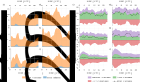
\includegraphics[width=39pc]{old_figures/error_decomp_sa.pdf}
%DIFDELCMD < %%%
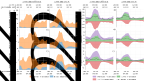
\includegraphics[width=39pc]{error_decomp_bris.pdf}
\DIFaddendFL \caption{Mean square error between the AWS and \DIFdelbeginFL \DIFdelFL{HRES }\DIFdelendFL \DIFaddbeginFL \DIFaddFL{official forecast }\DIFaddendFL zonal perturbations \DIFdelbeginFL \DIFdelFL{$\overline{\left(u_\text{AWS} - u_\text{H}\right)^2}$}\DIFdelendFL \DIFaddbeginFL \DIFaddFL{$\overline{\left(u_\text{AWS} - u_\text{O}\right)^2}$}\DIFaddendFL , a), e), and i), decomposed into the error variance \DIFdelbeginFL \DIFdelFL{$\var\left(u_\text{AWS} - u_\text{H}\right)$ }\DIFdelendFL \DIFaddbeginFL \DIFaddFL{$\var\left(u_\text{AWS} - u_\text{O}\right)$ }\DIFaddendFL and squared bias \DIFdelbeginFL \DIFdelFL{$\left(\overline{u}_\text{AWS} - \overline{u}_\text{H}\right)^2$ }\DIFdelendFL \DIFaddbeginFL \DIFaddFL{$\left(\overline{u}_\text{AWS} - \overline{u}_\text{O}\right)^2$ }\DIFaddendFL terms of equation (\ref{Eq:MSE}). Also, the decomposed mean square error between the AWS and \DIFdelbeginFL \DIFdelFL{official forecast }\DIFdelendFL \DIFaddbeginFL \DIFaddFL{OCF }\DIFaddendFL zonal perturbations, b), f) and j). Additionally, the \DIFdelbeginFL \DIFdelFL{HRES and }\DIFdelendFL AWS \DIFaddbeginFL \DIFaddFL{and official forecast }\DIFaddendFL error variance term \DIFdelbeginFL \DIFdelFL{$\var\left(u_\text{AWS} - u_\text{H}\right)$ }\DIFdelendFL \DIFaddbeginFL \DIFaddFL{$\var\left(u_\text{AWS} - u_\text{O}\right)$ }\DIFaddendFL decomposed into the $\var\left(u_\text{AWS}\right)$, \DIFdelbeginFL \DIFdelFL{$\var\left(u_\text{H}\right)$ }\DIFdelendFL \DIFaddbeginFL \DIFaddFL{$\var\left(u_\text{O}\right)$ }\DIFaddendFL and  \DIFdelbeginFL \DIFdelFL{$- 2 \cdot \cov\left(u_\text{AWS}, u_\text{H}\right)$ }\DIFdelendFL \DIFaddbeginFL \DIFaddFL{$- 2 \cdot \cov\left(u_\text{AWS}, u_\text{O}\right)$ }\DIFaddendFL terms, c), g) and k), and analogously for the official forecast and \DIFdelbeginFL \DIFdelFL{AWS }\DIFdelendFL \DIFaddbeginFL \DIFaddFL{OCF }\DIFaddendFL error variance term $\var\left(u_\text{AWS} - u_\text{O}\right)$, d), h) and l). Decompositions given for \DIFdelbeginFL \DIFdelFL{Adelaide }\DIFdelendFL \DIFaddbeginFL \DIFaddFL{Brisbane }\DIFaddendFL Airport, a) to d), the \DIFdelbeginFL \DIFdelFL{Adelaide }\DIFdelendFL \DIFaddbeginFL \DIFaddFL{Brisbane }\DIFaddendFL city station group, e) to h), and the \DIFdelbeginFL \DIFdelFL{SA }\DIFdelendFL \DIFaddbeginFL \DIFaddFL{Queensland }\DIFaddendFL coastal station group, i) to l)\DIFdelbeginFL \DIFdelFL{(see }\DIFdelendFL \DIFaddbeginFL \DIFaddFL{. See }\DIFaddendFL Fig.~\ref{Fig:map} \DIFaddbeginFL \DIFaddFL{for station locations}\DIFaddendFL .\DIFdelbeginFL \DIFdelFL{)}\DIFdelendFL }
\DIFdelbeginFL %DIFDELCMD < \label{Fig:error_decomp_sa}
%DIFDELCMD < %%%
\DIFdelendFL \label{Fig:error_decomp_bris}
\end{figure*}

Figure \DIFdelbegin \DIFdel{\ref{Fig:error_decomp_sa} }\DIFdelend \DIFaddbegin \DIFadd{\ref{Fig:error_decomp_bris} }\DIFaddend shows the terms of equation (\ref{Eq:MSE}) for both the official forecast and \DIFdelbegin \DIFdel{HRES for Adelaide }\DIFdelend \DIFaddbegin \DIFadd{OCF, for Brisbane }\DIFaddend Airport, the \DIFdelbegin \DIFdel{Adelaide }\DIFdelend \DIFaddbegin \DIFadd{Brisbane }\DIFaddend city station group, and the \DIFdelbegin \DIFdel{SA }\DIFdelend \DIFaddbegin \DIFadd{QLD }\DIFaddend coastal station group. At all three scales the official forecast varies more than \DIFdelbegin \DIFdel{HRES, which is also the case at the other locations }\DIFdelend \DIFaddbegin \DIFadd{OCF. The official forecast also generally varies more than ACCESS and HRES (not shown), and this is also true for the other stations and station groups }\DIFaddend considered in this study. 
\DIFdelbegin \DIFdel{At Adelaide }\DIFdelend \DIFaddbegin 

\DIFadd{At Brisbane }\DIFaddend airport the variance of AWS is significantly larger than either the official forecast or \DIFdelbegin \DIFdel{HRES, but this }\DIFdelend \DIFaddbegin \DIFadd{OCF. This }\DIFaddend additional variability is mostly uncorrelated to either dataset. \DIFdelbegin \DIFdel{This is }\DIFdelend \DIFaddbegin \DIFadd{Although the covariance between the official forecast and AWS increases between 20:00 and 08:00, the increase is not sufficient to offset the official forecast's additional variance, and the error variances are thus of comparable magnitude for both the official forecast and OCF. 
}

\DIFadd{The larger AWS variances are }\DIFaddend unsurprising from representation considerations alone \citep[e.g.][]{zaron06}, as the official forecast and \DIFdelbegin \DIFdel{HRES }\DIFdelend \DIFaddbegin \DIFadd{OCF }\DIFaddend data represent averages over 6 km spatial grid-cells, whereas the AWS data represent point values. As a result, error variance terms are \DIFaddbegin \DIFadd{generally }\DIFaddend much larger than the squared bias terms \DIFaddbegin \DIFadd{at this scale. The exception is OCF at 04:00, where the squared bias is $\approx 6$ kt, while error variance is $\approx 15$ kt. This results in a higher MSE for OCF than the official forecast around 04:00}\DIFaddend , \DIFdelbegin \DIFdel{and of comparable magnitudes for both datasets. This is }\DIFdelend consistent with the \DIFdelbegin \DIFdel{comparatively noisy DAE }\DIFdelend \DIFaddbegin \DIFadd{airport station $\overline{\text{DAE}}$ }\DIFaddend results of Figs.~\DIFdelbegin \DIFdel{\ref{Fig:airport_wpi} a) and b}\DIFdelend \DIFaddbegin \DIFadd{\ref{Fig:airport_DAE} c) and d}\DIFaddend ).

At the intermediate \DIFdelbegin \DIFdel{Adelaide }\DIFdelend \DIFaddbegin \DIFadd{Brisbane }\DIFaddend city station group scale, the AWS variances are \DIFdelbegin \DIFdel{of similar magnitudes to those of HRES, but smaller than }\DIFdelend \DIFaddbegin \DIFadd{again larger than those of OCF, but of comparable magnitude to }\DIFaddend those of the official forecast, with the official forecast's additional variability \DIFaddbegin \DIFadd{again }\DIFaddend mostly uncorrelated to AWS. This results in larger error variance terms for the official forecast, consistent with \DIFdelbegin \DIFdel{HRESs }\DIFdelend \DIFaddbegin \DIFadd{OCFs }\DIFaddend almost complete outperformance of the official forecast in Figs.~\DIFdelbegin \DIFdel{\ref{Fig:airport_wpi} }\DIFdelend \DIFaddbegin \DIFadd{\ref{Fig:city_DAE} c) and d). However, OCF's squared bias terms remain larger than the official forecast's, resulting in OCF's MSE slightly exceeding the official forecast's at around 04:00. These results are consistent with Figs.\ref{Fig:city_DAE} }\DIFaddend c) and d)\DIFdelbegin \DIFdel{. }\DIFdelend \DIFaddbegin \DIFadd{, where the official forecast slightly outperforms OCF at 04:00 with a confidence score of $79\%$.  
}

\DIFaddend Over the coarse \DIFdelbegin \DIFdel{SA }\DIFdelend \DIFaddbegin \DIFadd{QLD }\DIFaddend coastal station group scale, variances in all three datasets are \DIFdelbegin \DIFdel{now }\DIFdelend small enough that the error variance terms \DIFdelbegin \DIFdel{no longer dwarf }\DIFdelend \DIFaddbegin \DIFadd{are less dominant over }\DIFaddend the bias terms. Although the error variance of the official forecast is still larger than that of \DIFdelbegin \DIFdel{HRES, HRES}\DIFdelend \DIFaddbegin \DIFadd{OCF, OCF}\DIFaddend 's zonal biases \DIFdelbegin \DIFdel{at 05}\DIFdelend \DIFaddbegin \DIFadd{around 04}\DIFaddend :00 UTC are \DIFdelbegin \DIFdel{now }\DIFdelend \DIFaddbegin \DIFadd{again }\DIFaddend sufficient to result in \DIFdelbegin \DIFdel{a larger MSE at this time, consistent with the DAE results of Fig.~\ref{Fig:wpi_coastal} }\DIFdelend \DIFaddbegin \DIFadd{larger MSEs around this time. When considered with the analogous plots for the meridional perturbations (not shown), for which OCFs squared bias terms peak slightly later, the results are consistent with Figs.~\ref{Fig:coastal_DAE} }\DIFaddend c) and d). 

Analogous points can be made for the other locations \DIFaddbegin \DIFadd{and datasets }\DIFaddend considered in this study\DIFdelbegin \DIFdel{, the main exception being Darwin airport , Darwin city station group, and the NT }\DIFdelend \DIFaddbegin \DIFadd{. At the airport station scale, AWS variance is generally significantly higher than that of the official forecast and model guidance, producing high error variance and likely explaining why the airport station DAE results of Fig.~\ref{Fig:airport_DAE} are comparatively noisier than those of the city or }\DIFaddend coastal station group \DIFdelbegin \DIFdel{, where zonal biases in HREF around 01:00 - 03:00 UTC are large enough to overcome }\DIFdelend \DIFaddbegin \DIFadd{scales. Interesting exceptions include OCF at Brisbane and Perth airports, where amplitude biases in OCF's diurnal cycle are sufficient to affect airport station DAE scores.
}

\DIFadd{At the city station group scale, }\DIFaddend the official forecast \DIFdelbegin \DIFdel{'s larger error variance, producing the }\DIFdelend \DIFaddbegin \DIFadd{is generally outperformed by HRES and OCF in the $\overline{\text{DAE}}$ }\DIFaddend results of Fig.~\DIFdelbegin \DIFdel{\ref{Fig:airport_wpi} and Figs.~\ref{Fig:wpi_coastal} c) and d). The results of Fig.~\ref{Fig:airport_wpi} c) and d) are therefore generally a consequence of }\DIFdelend \DIFaddbegin \DIFadd{\ref{Fig:city_DAE}, and in the analogous comparisons with ACCESS (not shown). This occurs because }\DIFaddend the official forecast \DIFdelbegin \DIFdel{being }\DIFdelend \DIFaddbegin \DIFadd{is generally }\DIFaddend more variable than \DIFdelbegin \DIFdel{HRES, with }\DIFdelend \DIFaddbegin \DIFadd{model guidance, and }\DIFaddend this additional variability \DIFaddbegin \DIFadd{is }\DIFaddend mostly random, in the sense of being uncorrelated with AWS. \DIFdelbegin \DIFdel{Similarly, the official forecast is generally more variable than ACCESS, explaining why the official forecast also struggles to outperform ACCESS at these scales, and ACCESS is generally more variable than HRES, explaining why HRES generally outperforms ACCESS in the DAE results of Fig.~\ref{Fig:airport_wpi_EA}. In }\DIFdelend \DIFaddbegin \DIFadd{At }\DIFaddend the coastal station group \DIFdelbegin \DIFdel{DAE results of Fig.~\ref{Fig:wpi_coastal}, the }\DIFdelend \DIFaddbegin \DIFadd{scale, }\DIFaddend random variability in each dataset is reduced, and biases are \DIFdelbegin \DIFdel{now large enough to actually affect errors in the diurnal component of the forecast}\DIFdelend \DIFaddbegin \DIFadd{sufficiently large relative to error variance to affect the $\overline{\text{DAE}}$ results of Fig.~\ref{Fig:coastal_DAE}}\DIFaddend .

These results \DIFdelbegin \DIFdel{show }\DIFdelend \DIFaddbegin \DIFadd{suggest }\DIFaddend that switching model guidance products or performing edits can add more random noise to the diurnal component of the official forecast than what can be offset by reductions in bias, or improved correlations with AWS. Because the official forecast is built from multiple model \DIFdelbegin \DIFdel{datasets, most commonly HRES and ACCESS, blending }\DIFdelend \DIFaddbegin \DIFadd{guidance datasets, switching between }\DIFaddend datasets with different means will tend to produce greater variance than any of the component datasets. If the choice of model guidance is made primarily on which model best captures more slowly evolving\DIFaddbegin \DIFadd{, larger amplitude }\DIFaddend synoptic scale features, then switching model guidance may add random variability to the diurnal component of the official forecast. Furthermore, unless all forecasters follow identical thought processes when making edits, the edits will also add random variability. 
\DIFdelbegin \DIFdel{It is less clear why ACCESS shows greater random variability than HRES: one cause may be ACCESS's shorter time-step.  
}\DIFdelend 

These results \DIFaddbegin \DIFadd{could }\DIFaddend have implications for forecasting practice. Model guidance products are indeed biased in how they resolve diurnal wind cycles (e.g. Fig.~\ref{Fig:ellipse_hodo}), and there is therefore scope for forecaster edits to reduce these biases. However, editing model guidance generally fails to reduce error in the forecast diurnal \DIFdelbegin \DIFdel{cycle}\DIFdelend \DIFaddbegin \DIFadd{signal}\DIFaddend , even at scales finer than the effective resolutions of the models, as \DIFdelbegin \DIFdel{the cycle itself is mostly hidden }\DIFdelend \DIFaddbegin \DIFadd{at these scales diurnal cycles are significantly masked }\DIFaddend by random variability. Averaging over large areas reduces this random variability, \DIFaddbegin \DIFadd{better revealing the diurnal cycle, }\DIFaddend and so biases have a greater impact on forecast error\DIFdelbegin \DIFdel{, but }\DIFdelend \DIFaddbegin \DIFadd{. However, }\DIFaddend even at large scales Fig.~\DIFdelbegin \DIFdel{\ref{Fig:wpi_coastal} }\DIFdelend \DIFaddbegin \DIFadd{\ref{Fig:coastal_DAE} }\DIFaddend shows model guidance still outperforms the official forecast more often than not.

Reducing the random variability of the official forecast, or the model guidance datasets that comprise it, \DIFdelbegin \DIFdel{will }\DIFdelend \DIFaddbegin \DIFadd{could }\DIFaddend therefore improve the capacity of these types of edits to reduce error \DIFaddbegin \DIFadd{in the diurnal cycle}\DIFaddend . One way to \DIFdelbegin \DIFdel{do }\DIFdelend \DIFaddbegin \DIFadd{accomplish }\DIFaddend this would be to \DIFdelbegin \DIFdel{move to an ensemble forecasting system}\DIFdelend \DIFaddbegin \DIFadd{use an ensemble average model guidance product like OCF}\DIFaddend , another would be to \DIFaddbegin \DIFadd{further }\DIFaddend post process model guidance products, such as by averaging multiple time steps around the hour, before including them in \DIFaddbegin \DIFadd{the }\DIFaddend GFE.

\section{Conclusion}
\label{Sec:Conclusion}
In this study \DIFdelbegin \DIFdel{we }\DIFdelend \DIFaddbegin \DIFadd{I }\DIFaddend have presented methods for \DIFdelbegin \DIFdel{verifying }\DIFdelend \DIFaddbegin \DIFadd{assessing }\DIFaddend the diurnal component of wind forecasts, with the intended application being the assessment of the edits Australian forecasters make to model guidance datasets \DIFdelbegin \DIFdel{in order }\DIFdelend to better resolve land-sea breeze and boundary layer mixing processes. \DIFdelbegin \DIFdel{We }\DIFdelend \DIFaddbegin \DIFadd{I }\DIFaddend considered both errors and seasonal biases at each hour UTC, over three spatial scales, but the methods are immediately generalisable to other spatiotemporal scales. 

When the methods are applied to Australian forecast data, the results indicate that the official edited forecast only produces lower absolute errors in the diurnal wind \DIFdelbegin \DIFdel{cycle when averaged over coarse spatial scales of $500\times 150$ km$^{2}$ to $2000 \times 150$ km$^{2}$: this scale corresponds to the aggregation of data within 150 km of the Australian coastline, subdivided into linear segments of coastline and by state }\DIFdelend \DIFaddbegin \DIFadd{signal when wind perturbation data is averaged over the coarse ``coastal station group" spatial scale }\DIFaddend (see Fig.~\ref{Fig:map}) \DIFaddbegin \DIFadd{of $500\times 100$ km$^{2}$ to $2000 \times 100$ km$^{2}$}\DIFaddend . Even at these scales, reductions in error are isolated to particular locations and times of day, and the official forecast rarely has lower mean absolute error than \DIFdelbegin \DIFdel{both commonly used model guidance products simultaneously. This suggests that forecaster skill in improving diurnal wind processes lies more in making the choice of model guidance than in making edits}\DIFdelend \DIFaddbegin \DIFadd{the three model guidance products considered in this study simultaneously}\DIFaddend .

By contrast, the official forecast can produce lower seasonal biases than model guidance at all three spatial scales, but again, it rarely produces lower biases than \DIFdelbegin \DIFdel{both standard }\DIFdelend \DIFaddbegin \DIFadd{the three }\DIFaddend model guidance products \DIFaddbegin \DIFadd{considered here }\DIFaddend simultaneously. Reduced seasonal biases do not translate into reduced errors at the two smaller spatial scales because the diurnal cycle is mostly masked by the random variability in each dataset. Furthermore, because the official forecast \DIFaddbegin \DIFadd{generally }\DIFaddend exhibits much greater random variability than \DIFdelbegin \DIFdel{HRES, HRES }\DIFdelend \DIFaddbegin \DIFadd{model guidance, model guidance }\DIFaddend almost uniformly outperforms the official forecast over the intermediate $50\times 50$ km$^{2}$ to $200 \times 200$ km$^{2}$ \DIFaddbegin \DIFadd{city station group }\DIFaddend spatial scale.
\DIFdelbegin \DIFdel{The same is true for ACCESS, although to a slightly lesser extent, and also explains why HRES mostly outperforms ACCESS at this scale. 
}\DIFdelend 

\DIFdelbegin \DIFdel{We }\DIFdelend \DIFaddbegin \DIFadd{I }\DIFaddend also compare structural features of the \DIFaddbegin \DIFadd{mean }\DIFaddend diurnal wind cycles of each dataset by fitting modified ellipses to \DIFdelbegin \DIFdel{hodographs of seasonally averaged diurnal wind cycles}\DIFdelend \DIFaddbegin \DIFadd{their temporal hodographs}\DIFaddend , then deriving metrics from these ellipses. This approach reveals structural biases in the official forecast, including directional biases in the approach of the sea-breeze at Brisbane airport, \DIFdelbegin \DIFdel{eccentricity biases along the coast of NSW, }\DIFdelend and amplitude biases along the southwest coast of \DIFdelbegin \DIFdel{WA. It also reveals biases in model guidance datasets, such as ACCESS's overemphasis of boundary layer mixing processes around Hobart}\DIFdelend \DIFaddbegin \DIFadd{Western Australia}\DIFaddend .

Future research could extend this study in multiple directions.  One \DIFaddbegin \DIFadd{approach would be to study how the difference of absolute errors (DAE) metric defined in this study responds to synthetic, or idealised model data, so that the influence of random and synoptic variability can be better understood: some preliminary work to this end is available online \mbox{%DIFAUXCMD
\citep{short20}}\hspace{0pt}%DIFAUXCMD
. Another }\DIFaddend important question is whether the random variability in the official forecast, or the model guidance products that comprise it, \DIFdelbegin \DIFdel{could }\DIFdelend \DIFaddbegin \DIFadd{can }\DIFaddend be reduced through ensemble forecasting or post-processing, as reducing random variability would both decrease errors, and \DIFaddbegin \DIFadd{could }\DIFaddend increase the value of land-sea breeze and boundary layer mixing edits. \DIFaddbegin \DIFadd{The BoM's Operational Consensus Forecast (OCF) is an effective way to accomplish this, and future work could assess whether it is possible, or desirable, to adjust OCF's wind algorithm to reduce the amplitude biases identified in OCF's mean diurnal cycle, noting that these biases are subject to how the mean diurnal cycle has been defined in this study. }\DIFaddend Another goal could be to identify precisely the spatiotemporal scales at which diurnal wind cycles can be \DIFdelbegin \DIFdel{identified against background noise}\DIFdelend \DIFaddbegin \DIFadd{separated from random variability}\DIFaddend , so as to better understand the scales at which land-sea breeze and boundary layer mixing edits can \DIFdelbegin \DIFdel{add value to }\DIFdelend \DIFaddbegin \DIFadd{reduce error in }\DIFaddend a forecast.

\acknowledgments
Funding for this study was provided for Ewan Short by the Australian Research Council's Centre of Excellence for Climate Extremes (CE170100023). Datasets and software were generously provided by the Australian Bureau of Meteorology's Evidence Targeted Automation team, with additional code available online \citep{shortGitVeri19}. Thanks are due to Michael Foley, Deryn Griffiths, Nicholas Loveday, Ben Price and Alexei Hider for providing support at the Bureau of Meteorology's Melbourne and Darwin offices, and to \DIFdelbegin \DIFdel{Professors Craig Bishopand Todd Lane }\DIFdelend \DIFaddbegin \DIFadd{Craig Bishop, Todd Lane and Claire Vincent }\DIFaddend from the University of Melbourne, and Carly Kovacik from the United States' National Weather Service, for some helpful conversations. 
\DIFaddbegin 

\DIFaddend \bibliographystyle{ametsoc2014}
\bibliography{./references.bib}

\end{document}
